%=======================================================================
% CSE465 Final Report --- North South University
%
% BUILD: pdfLaTeX on Overleaf. Order: pdflatex -> bibtex -> pdflatex x2
%
%======================================================================
\documentclass[journal,onecolumn]{IEEEtran}

\usepackage{graphicx}
\usepackage{amsmath}
\usepackage{amssymb}
\usepackage{booktabs}
\usepackage{multirow}
\usepackage{array}
\usepackage{url}
\usepackage[hidelinks]{hyperref}

\newcommand{\best}[1]{\textbf{#1}}
\newcommand{\notrun}{\textsc{not run}}
\newcommand{\notrec}{\textsc{not recoverable}}

\setcounter{topnumber}{4}
\setcounter{bottomnumber}{3}
\setcounter{totalnumber}{6}
\renewcommand{\topfraction}{0.92}
\renewcommand{\bottomfraction}{0.9}
\renewcommand{\textfraction}{0.05}
\renewcommand{\floatpagefraction}{0.7}

\begin{document}

\title{Auditing the Score Before the Model: Corrected Evaluation
Baselines and a Pre-Registered Negative Result for Respiratory Sound
Classification on ICBHI 2017}

\author{Barshon~Basak,~Asif~Mahbub,~Sami~Uddin,~and~Farhana~Rahman%
\thanks{The authors are with the Department of Electrical and Computer
Engineering, North South University, Dhaka, Bangladesh. Course: CSE465,
Machine Learning. Supervisor: Dr.~Riasat Khan.}}

\maketitle

%=======================================================================
\begin{abstract}
Respiratory sound classification is judged almost everywhere on one public lung sound
benchmark, and almost every system is ranked by a single headline score. This project set out
to build a better classifier and ended up asking a prior question: how much of that score
belongs to the model, and how much to the way it was measured. We audited our own
pipeline of 39 experiments and found five faults in the measurement itself, each recovered
from a stored prediction table. A wrongly averaged score
variant inflated 20 runs by 9.5 points on average and 22 at worst. A split loader that
silently fell back to a patient identifier rule produced a test partition of 11 patients
while recording itself as the official one, worth almost 9 points alone. The published
partition assigns recordings instead of patients, so two patients sit on both sides, though
repairing that leak moves the score by four tenths of a point. One recording carries a device
suffix the released audio does not, so a naive join drops it silently. Choosing the saved
model by training loss rather than by the challenge score costs 7 to 10 points across three
seeds. Under a corrected protocol we segment every breathing cycle, convert it to a log scaled
spectrogram, and train one lightweight convolutional network and three pretrained vision
transformers, reporting accuracy, precision, recall, sensitivity, specificity, parameter
count, size and training time for each, with and without spectrogram masking.
A fourth transformer, pretrained on general audio before the audit, stored no prediction
table and is reported as unrecoverable. The best model is then examined
with a twelve row ablation study, a three seed noise floor, paired patient level tests, and
explainable artificial intelligence. The contribution is a measurement, not a mechanism.
\end{abstract}

\begin{IEEEkeywords}
Ablation study, convolutional neural network, data augmentation, evaluation protocol,
explainable artificial intelligence, ICBHI 2017, label reliability, pre-registration,
reproducibility, respiratory sound classification, transfer learning, vision transformer.
\end{IEEEkeywords}

%=======================================================================
\section{Introduction}
\label{sec:intro}

Listening to the chest with a stethoscope is still the first thing a doctor does when a
patient arrives short of breath, and it is also one of the least reproducible things a
doctor does. The sounds that matter clinically---crackles, which are short popping
transients, and wheezes, which are longer musical tones---are quiet, easily buried under
heart sounds and room noise, and described by different physicians in different words.
Automating their detection is an obvious target for machine learning, and the ICBHI 2017
Respiratory Sound Database~\cite{rocha2019icbhi} has become the standard place to try. We
picked this problem for our capstone because the benchmark is mature. A brand new
architecture was never going to move it far, which made it a reasonable place to ask a
different kind of question. The question we ended up asking is whether the scores the
field reports on this corpus mean what everybody takes them to mean, and we started by
asking it of ourselves.

\subsection{Literature Review}
\label{subsec:lit}

Each member of the group reviewed at least one journal paper. The reviews are consolidated
here in the order they became relevant to our own design.

\textbf{Where the benchmark stands.} Yu \emph{et al.}~\cite{electronics2025review} review 135
technical publications built on this one database and separate the two tasks it supports:
recognising the pathological state of a patient, where several systems exceed 98 percent
accuracy, and categorising the adventitious sound in a single cycle, which remains much harder
because of severe class imbalance. Their recommendation---more interpretable models and better
use of the data that surrounds the audio---is the direction most recent work has taken. The
pattern within that literature is that progress since roughly 2021 has come from better
pretraining rather than better architecture: convolutional systems pretrained on
ImageNet~\cite{deng2009imagenet} plateau near 0.56 on the official challenge
metric~\cite{respirenet2021}, while transformers pretrained on
AudioSet~\cite{gemmeke2017audioset} sit five to nine points
higher~\cite{bae2023patchmix,bts2024,pafa2025}. Suma \emph{et al.}~\cite{suma2025mtl} attack
both tasks at once with a single-input multi-output network over mel-frequency cepstral
coefficients, comparing four backbones and finding a MobileNet best at 74 percent on sounds and
91 percent on diseases---without stating which partition those numbers are on, which is the
first sign of the problem this paper is about. Two 2025 fusion
systems~\cite{adffnet2025,bspc2025fusion} report gains of roughly one point, the scale at which
the measurement questions below start to matter.

\textbf{What pretraining is worth, and what the recording conditions cost.} Bae
\emph{et al.}~\cite{bae2023patchmix} fine-tune an Audio Spectrogram
Transformer~\cite{gong2021ast} with a patch-mixing contrastive objective and reach 0.6237,
while Niizumi \emph{et al.}~\cite{frozenfm2025} freeze the audio foundation model entirely,
train only a linear probe, and still reach 0.5938---above several fully fine-tuned
convolutional systems. Most of the useful information therefore sits in the pretrained
representation rather than the fine-tuning, provided the pretraining was on audio. Moummad and
Farrugia~\cite{scl2023} reach 0.5755 with a small CNN and contrastive pretraining on metadata,
and Nguyen and Pernkopf~\cite{nguyen2022cotuning} add that transfer from ImageNet to
spectrograms is fragile and needs regularisation. Kim \emph{et al.}~\cite{kim2025metadata}
push the metadata idea furthest and reach a conclusion we had to confront directly: they
evaluate recording device, chest location, sex and age as sources of domain shift, use the most
informative combinations to guide a supervised contrastive objective, and identify
recording-condition bias as a primary limiting factor for models trained on this corpus.
Section~\ref{subsec:dataset} reports what we found when we went looking for that axis in the
data itself.

\textbf{Interpretability and open-world behaviour.} Concept bottleneck
models~\cite{koh2020cbm} route a prediction through human-named concepts so the reasoning
can be inspected, which is attractive here because crackles and wheezes have physical
definitions; this was our original plan. Karim \emph{et al.}~\cite{karim2024mosquito}, from
our own department, combine vision transformers with OpenMax rejection, which we
reimplemented as our open-set baseline, and knowledge distillation with a teaching
assistant~\cite{pavel2024kd} gave us the compression arm. Yang
\emph{et al.}~\cite{yang2024ood} supply the vocabulary separating out-of-distribution
detection from open-set recognition and Kejriwal \emph{et al.}~\cite{kejriwal2024owl} the
staged open-world protocol, while Cho and Lee~\cite{cho2025openset}---the only group we found
doing open-set recognition on respiratory audio---report an improvement over a semi-supervised
baseline rather than an absolute score. Cruz \emph{et al.}~\cite{cruz2025owl}, surveying what
the open-world field still has not solved, group the open problems into the theory of novelty,
the design of agents, and their evaluation---and it is the third group, where they name
inconsistent evaluation metrics as an unresolved issue, that turned out to describe our
situation rather than the first two.

\textbf{How well humans do the same task.} This was the most important group we read.
Tzeng \emph{et al.}~\cite{tzeng2025jmir} had seven senior physicians blindly annotate a
quarter of the ICBHI test set; on clean audio they reached an ICBHI score of 47.77 percent
at a sensitivity of 23.23 percent, with mean self-rated confidence 2.88 out of 5. Melbye
\emph{et al.}~\cite{melbye2016kappa} had twelve physicians classify twenty reference
recordings and found agreement below $\kappa = 0.40$ for detailed descriptions, rising to
0.62 and 0.59 when crackles and wheezes are collapsed to simple presence. Huang
\emph{et al.}~\cite{huang2024crackles} report a larger clinical archive where agreement on
wheeze is very high ($\kappa = 0.948$) but on crackle only moderate ($\kappa = 0.516$). The
three disagree on the level and agree on the shape: crackle labels are far less reliable than
wheeze labels, and reliability falls sharply as the description gets finer. Against that
background, Bikku \emph{et al.}~\cite{scirep2025cnnrnn} fuse a convolutional encoder with a
recurrent one over mel-spectrograms drawn from two corpora, map crackles to pneumonia and
wheezes to obstructive disease, explain the result with gradient, Shapley and local surrogate
methods, and report 94.0 percent accuracy under five-fold cross-validation. The explanations
are aligned to the same cycle labels the three studies above characterise, and the partition is
not the official one, so the number cannot be read against the systems in the first block. Both
observations shaped how we report our own interpretability results in
Section~\ref{subsec:xai}.

\subsection{Gaps in the Related Work}
\label{subsec:gaps}

Reading the two groups side by side exposed four gaps we could act on.

First, \emph{the reported score is treated as a property of the model}. Papers in the first
group report one composite number and compare it against other papers' composite numbers; few
state which of the circulating definitions they used, and the partition is often described
loosely or not at all---the multi-task study above does not name one, and the
convolutional-recurrent study reports five-fold cross-validation, which is a perfectly clear
choice that simply cannot be read against the official-split numbers beside it. We could not
find an ICBHI paper that ablates its evaluation protocol the way it ablates its architecture,
even though our audit shows the protocol is worth more than any architectural choice we made.

Second, \emph{the official split is assumed to be patient-independent and it is not}. The
published file assigns recordings, not patients, and two patients have recordings on both
sides---a validity fault no paper we read mentions.

Third, \emph{the reference standard is never characterised}. The first group validates models
against ICBHI's cycle labels; the second shows those labels are reproduced by trained
physicians at 47.77 percent and agreed on at $\kappa$ well below 0.40 for fine distinctions. A
detector scored against a reference standard of unknown reliability produces a number of
unknown meaning.

Fourth, \emph{negative results are missing}. We could not find a paper that fixed a validity
threshold in advance, ran against it, and reported the failure---without which a reader cannot
tell how many attempts a reported success survived.

\subsection{Our Work}
\label{subsec:ourwork}

We started with an open-world multi-task design: a shared spectrogram backbone, one head for
the four sound-event classes and one for disease, with a bottleneck of physics-derived acoustic
concepts in between. We set a gate before building it: the extractors had to reproduce ICBHI's
crackle and wheeze labels at an area under the curve of at least 0.65, with an interval
excluding chance, measured once per run on the test partition, and two runs were budgeted. Both
failed---0.5506 then 0.5580 for crackle, 0.5729 then 0.5340 for wheeze---and we stopped, as the
gate said we would.

That failure sent us back to look at how we were measuring anything, and the audit turned
up five faults in our own evaluation, priced in Section~\ref{subsec:protocol}. Correcting
them moved our headline number from 0.7077 to 0.5602. That gap, 0.1475, is larger than the
effect of ImageNet pretraining, larger than the effect of augmentation, and larger than the
spread between our best and worst backbone. What we deliver is therefore not a mechanism
but a measurement: a corrected protocol, baselines produced under it, and tooling that
makes each fault detectable by somebody else.

We then rebuilt the model side under that protocol. One ImageNet-pretrained convolutional
network and three ImageNet-pretrained vision
transformers~\cite{dosovitskiy2021vit,liu2021swin,touvron2021deit} were trained on identical
inputs with identical schedules, each clean and with SpecAugment~\cite{park2019specaugment}. A
fourth transformer, an Audio Spectrogram Transformer~\cite{gong2021ast} pretrained on AudioSet,
had been run earlier in the project; it predates the audit and stored no prediction table, so
its challenge-metric score cannot be recovered, and Section~\ref{subsec:ast} reports that
rather than repairing it because it is the clearest illustration of the paper's own argument.
The best model, MobileNetV2~\cite{sandler2018mobilenetv2} with SpecAugment, was taken apart
with a twelve-row ablation, a three-seed noise floor, paired patient-level tests, and gradient-
and occlusion-based attribution~\cite{selvaraju2017gradcam}. Every transformer lost to the
convolutional baseline and the largest collapsed to the majority class; we report that rather
than tuning until it stops being true. Finally we returned to the concept question with a
fairer instrument, and it refuted the explanation we had begun to prefer
(Section~\ref{subsec:ceiling}).

The novelty here is not a layer or a loss. It is (i) an ablation of the evaluation protocol
itself, which we have not seen done on this benchmark; (ii) the identification of the
checkpoint selection rule as a first-class pipeline component, worth more than pretraining
or augmentation; (iii) a measured run-to-run noise floor used as an admissibility threshold
for every ablation delta we report; (iv) a pre-registered gate that failed, followed by a
pre-registered ceiling estimate that refuted our own account of why it failed; and (v) an
attribution analysis that contradicts the story the score tells and directly motivated one
of the ablation rows.

Section~\ref{sec:system} covers the corpus, partitions, preprocessing and models; no results
appear there. Section~\ref{sec:results} holds everything numeric, ending with the ablation
study in Section~\ref{subsec:ablation} and the comparison against published work in
Section~\ref{subsec:comparison}. Section~\ref{sec:conclusion} states what we would do next,
and Appendix~\ref{app:runmap} maps every model in this paper to the run identifier it
carries in our repository.

%=======================================================================
\section{Proposed System}
\label{sec:system}

Everything numeric that is a \emph{result} is held back for Section~\ref{sec:results}; the
counts here are properties of the data. Fig.~\ref{fig:flowchart} is the flowchart of the
complete system and doubles as a map of where each of the five faults of
Section~\ref{subsec:protocol} sits.

\begin{figure}[!t]
\centering
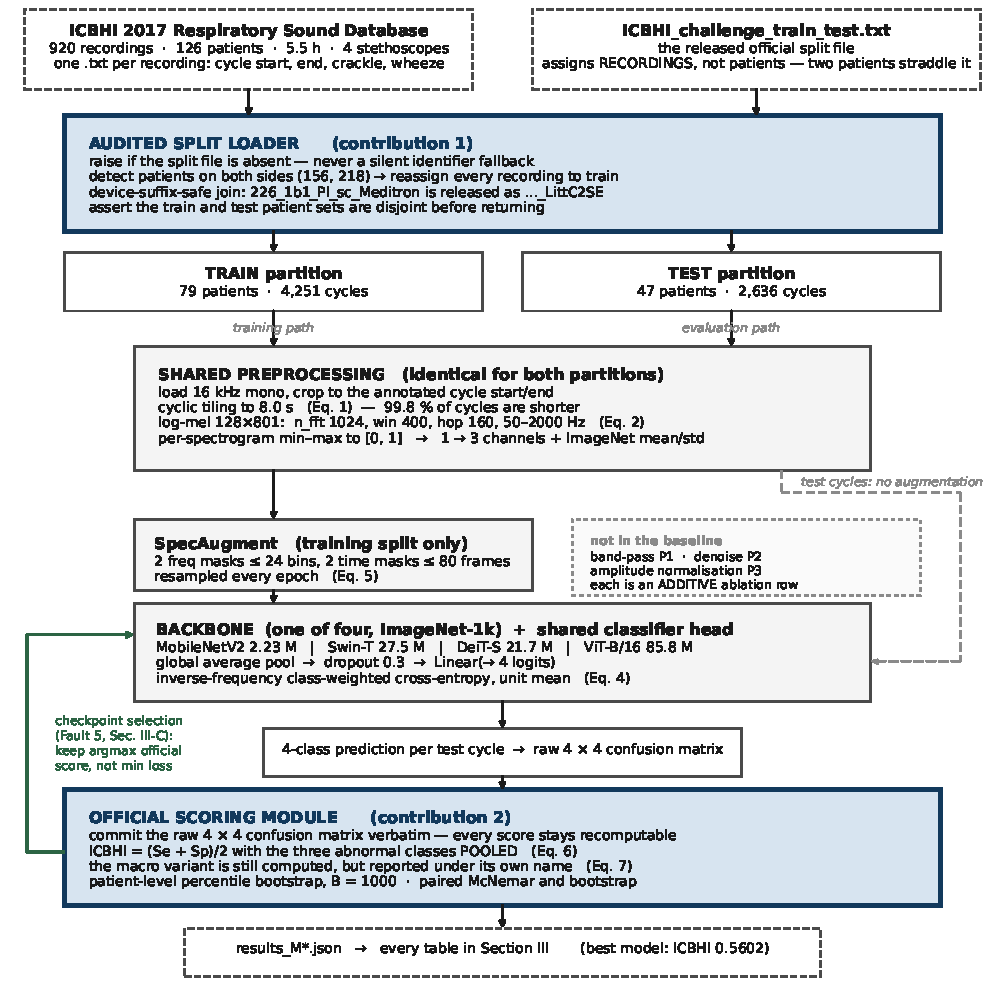
\includegraphics[width=0.38\linewidth]{figures/fig_flowchart.pdf}
\caption{Flowchart of the complete system. Audio is segmented into annotated respiratory
cycles, standardised in length, converted to a log-mel spectrogram and classified into four
sound-event classes. The split loader, the metric definition and the checkpoint selection
rule are treated as pipeline components with their own ablation rows rather than as fixed
infrastructure.}
\label{fig:flowchart}
\end{figure}

\subsection{Dataset}
\label{subsec:dataset}

We use the ICBHI 2017 Respiratory Sound Database~\cite{rocha2019icbhi} from its public
release: 920 recordings from 126 patients, annotated per respiratory cycle with a start time,
an end time, a crackle flag and a wheeze flag. Combining the two flags gives the four
sound-event classes used throughout---Normal, Crackle, Wheeze and Both---over 6,898 annotated
cycles with a median length of 2.42~s, which we standardise to an 8.0~s network input.
Recordings were captured with four stethoscopes at several chest locations at mixed sample
rates, which we resample to 16~kHz mono.

Two structural facts about the corpus shaped the project and are worth stating before any
result. Each patient carries a single diagnosis label, and those labels are extremely
imbalanced: COPD alone covers 64 of the 126 patients and 83.3 percent of all cycles, which is
why the disease side of our original two-head design was eventually dropped from the headline.
And only 4 patients (112, 158, 218 and 226) were recorded on more than one device, so device
identity is almost perfectly confounded with patient identity. That is worth stating plainly
because Kim \emph{et al.}~\cite{kim2025metadata} identify recording-condition bias as a
primary limiting factor for models trained here: the axis they show matters is one this corpus
cannot be used to measure from the inside, since separating device from patient would require
patients recorded on several devices and there are four. It is a reason to take their
cross-dataset approach seriously, not a reason to doubt it.

\subsubsection{Partitions and class balance}
Table~\ref{tab:partitions} gives the three partitions this paper uses together with the
class composition of each. The published split file assigns \emph{recordings}, not patients,
so patients 156 and 218 have recordings on both sides. Our corrected partition moves every
recording of a leaking patient into the training side, which is the conservative direction:
the test side is then guaranteed to contain no patient the model has trained on. The repair
costs 12 of 381 test recordings and moves the ratio from 58.6/41.4 to 59.9/40.1, marginally
closer to the nominal 60/40 than the published file itself. All new results in this paper
are on the corrected partition; the other two appear only where a comparison demands it, and
always by name.

The imbalance is severe. On the corrected test partition the Both class holds 86 cycles
against 1,560 Normal, which is why every model here trains with the inverse-frequency
weighted loss of~(\ref{eq:weights}), and why accuracy is a misleading headline on this
corpus: always predicting Normal scores 0.5918 accuracy on that partition, higher than the
accuracy of our best model.

\begin{table}[!t]
\centering
\caption{The three partitions used in this paper with the class composition of each, computed
from the ICBHI annotation files and cross-checked against the committed confusion matrix of the
corresponding run. Spectrogram masking operates in place and adds no samples, so the augmented
training total equals the clean one.}
\label{tab:partitions}
\footnotesize
\begin{tabular}{llrrrrrrrr}
\toprule
Partition & Subset & Normal & Crackle & Wheeze & Both & Total & Aug.\ total & Patients & Rec. \\
\midrule
Whole corpus & --- & 3{,}642 & 1{,}864 & 886 & 506 & 6{,}898 & --- & 126 & 920 \\
\midrule
\multirow{2}{*}{\best{Corrected (ours)}}
 & Train & 2{,}082 & 1{,}247 & 513 & 420 & 4{,}262 & 4{,}262 & 79 & 551 \\
 & Test  & 1{,}560 & \phantom{0,}617 & 373 & \phantom{0}86 & 2{,}636 & --- & 47 & 369 \\
\midrule
\multirow{2}{*}{Published, verbatim}
 & Train & 2{,}063 & 1{,}215 & 501 & 363 & 4{,}142 & 4{,}142 & 77 & 539 \\
 & Test  & 1{,}579 & \phantom{0,}649 & 385 & 143 & 2{,}756 & --- & 49 & 381 \\
\midrule
\multirow{2}{*}{Identifier fallback}
 & Train & 3{,}387 & 1{,}700 & 848 & 471 & 6{,}406 & 6{,}406 & 115 & --- \\
 & Test  & \phantom{0,}255 & \phantom{0,}164 & \phantom{0}38 & \phantom{0}35 & \phantom{2,}492 & --- & \phantom{0}11 & --- \\
\bottomrule
\end{tabular}

\vspace{2pt}
\footnotesize The corrected partition reassigns the two leaking patients to training; the
published partition is the split file verbatim; the identifier-fallback partition is not a
design but a fault (Section~\ref{subsec:protocol}). Two earlier backbone runs use a fourth
policy that instead \emph{drops} the leaking patients' training recordings and leaves the
published test set byte-identical, so their test row is the published test row. Pooling the
abnormal classes, the corrected test partition holds 703 crackle-positive and 459
wheeze-positive cycles, the denominators of every concept result in
Section~\ref{subsec:gate}. One recording named \texttt{226\_1b1\_Pl\_sc\_Meditron} in the
split file is released as \texttt{226\_1b1\_Pl\_sc\_LittC2SE}, so a stem join drops it and its
11 cycles; it is a training recording, which is why our pipeline indexes 4,251 training cycles
where the annotations hold 4,262.
\end{table}

\subsection{Dataset Preprocessing}
\label{subsec:preprocessing}

The chain is implemented once and every stage is switchable, so the ablation of
Section~\ref{subsec:ablation} changes one thing at a time. In execution order it is: load and
resample to 16~kHz mono; optionally band-pass filter with a zero-phase fourth-order Butterworth
between 50 and 2000~Hz; segment into cycles at the annotated start and end times; standardise
every cycle to $T = 8.0$~s by cyclic tiling, (\ref{eq:tile}); optionally normalise each cycle
to unit peak amplitude; optionally denoise by spectral gating at the 25th percentile with an
over-subtraction factor of two; compute a log-mel spectrogram, (\ref{eq:logmel}), with 128 mel
bands, a 1024-point FFT, hop 160 and window 400 over 50--2000~Hz; rescale each spectrogram to
the unit interval, (\ref{eq:minmax}); replicate to three channels for the pretrained backbones;
encode the label as (\ref{eq:label}); handle imbalance in the loss, (\ref{eq:weights}); and
apply spectrogram masking, (\ref{eq:specaug}), to the training split only.

Three of those stages---band-pass filtering, denoising and per-cycle amplitude
normalisation---are \emph{off} in the reference configuration. That is deliberate. Turning
any of them on in the reference would silently move the baseline that every other ablation
delta is measured against, so instead they are switched on one at a time as rows
\texttt{P1}, \texttt{P2} and \texttt{P3} of Table~\ref{tab:ablation}, and their deltas
therefore read in the opposite direction to every other row: a positive delta is a
recommendation to adopt the stage.

The median cycle is 2.42~s against an 8.0~s input, so almost every cycle has to be extended.
We tile rather than pad with silence: for a cycle $x$ of length $L$ and a target of
$N = T f_s$ samples,

\begin{equation}
\tilde{x}[n] = x[n \bmod L], \qquad n = 0,\dots,N-1,
\label{eq:tile}
\end{equation}

and a longer cycle is cropped from the start. Tiling is common practice here, but it repeats
the same acoustic event two or three times inside one input and leaves a discontinuity at each
seam; row \texttt{P4} tests the alternative, for reasons Section~\ref{subsec:xai} supplies.
The tiled waveform becomes a log-mel spectrogram, with $X[m,k]$ the short-time Fourier
transform and $H_j[k]$ the $j$-th mel filter:

\begin{equation}
S[j,m] = 10\log_{10}\!\left(\frac{\sum_{k} H_j[k]\,\lvert X[m,k]\rvert^{2}}
{\displaystyle\max_{j',m'}\ \sum_{k} H_{j'}[k]\,\lvert X[m',k]\rvert^{2}}\right).
\label{eq:logmel}
\end{equation}

The maximum is per spectrogram, not global, which is itself a normalisation and is why the
explicit rescaling that follows is nearly free in the ablation. That rescaling is a min--max
map to the unit interval,

\begin{equation}
\tilde{S} = \frac{S - \min S}{\max S - \min S + \epsilon}, \qquad \epsilon = 10^{-8}.
\label{eq:minmax}
\end{equation}

Labels come from the two annotation flags, with $c$ the crackle flag and $w$ the wheeze flag,
both in $\{0,1\}$:

\begin{equation}
y = c + 2w \in \{0,1,2,3\} \;\equiv\; \{\text{Normal},\ \text{Crackle},\ \text{Wheeze},\ \text{Both}\}.
\label{eq:label}
\end{equation}

Imbalance is handled in the loss rather than by resampling, so the training distribution is
identical across every model and ablation row. For class $c$ with $N_c$ of $N$ training cycles
and $C = 4$, the raw inverse-frequency weight is renormalised to unit mean:

\begin{equation}
w_c = \frac{N}{C N_c} \bigg/ \frac{1}{C}\sum_{c'=1}^{C}\frac{N}{C N_{c'}},
\qquad
\mathcal{L} = -\frac{1}{B}\sum_{i=1}^{B} w_{y_i}\log p_{i,y_i}.
\label{eq:weights}
\end{equation}

The renormalisation is not cosmetic: without it the loss scale moves with the class
distribution and ablation rows that change the training set stop being comparable to the
reference. Augmentation is SpecAugment~\cite{park2019specaugment} on training spectrograms
only, with the same seed as the paired clean run so the two differ in one thing:

\begin{equation}
\tilde{S}[j,m] \leftarrow 0 \ \ \text{for}\ j \in [f_0, f_0{+}f),\ f \sim \mathcal{U}[0,24],
\ \ \text{and}\ m \in [t_0, t_0{+}t),\ t \sim \mathcal{U}[0,80],
\label{eq:specaug}
\end{equation}

two frequency masks and two time masks per spectrogram.

\subsection{Applied Models}
\label{subsec:models}

Table~\ref{tab:models} lists every model with its owner. The four backbones trained under the
corrected protocol share the same spectrograms, loss, partition, batch size of 16, cap of 40
epochs and seed 42, since anything else would turn the comparison into a comparison of tuning
effort; only the classifier head is replaced. The two families do differ in optimiser settings,
and we state that rather than smoothing it over: the convolutional model uses Adam at a single
learning rate of $5\times10^{-4}$ with dropout 0.3 and gradient clipping at 5.0, while the
vision transformers use AdamW at $10^{-4}$ on the backbone and $10^{-3}$ on the head, the
standard recipe for fine-tuning a pretrained transformer. Both use cosine annealing and weight
decay $10^{-4}$, and the ablation harness reuses the convolutional settings unchanged.

\begin{table}[!t]
\centering
\caption{Every model in this paper, with the group member who owned it. The four backbones
of the first block take the same $128 \times 801$ log-mel input replicated to three
channels, and each was run twice, clean and with spectrogram masking.}
\label{tab:models}
\footnotesize
\begin{tabular}{lllll}
\toprule
Backbone & Family & Pretraining & Owner & Protocol and status \\
\midrule
MobileNetV2~\cite{sandler2018mobilenetv2} & CNN & ImageNet & Asif Mahbub & corrected; complete \\
ViT-B/16~\cite{dosovitskiy2021vit} & Transformer & ImageNet-21k & Barshon Basak & corrected; complete \\
Swin-T~\cite{liu2021swin} & Transformer & ImageNet & Farhana Rahman & corrected; complete \\
DeiT-S~\cite{touvron2021deit} & Transformer & ImageNet & Sami Uddin & corrected; complete \\
\midrule
AST~\cite{gong2021ast} & Transformer & ImageNet + AudioSet & Asif Mahbub, Barshon Basak & pre-audit; score \notrec \\
2D-CNN, 4 blocks & CNN & from scratch & Asif Mahbub & alternative partition; reference \\
MobileNetV3-Small & CNN & ImageNet & Asif Mahbub & alternative partition; reference \\
MobileNetV2 ensemble, $N{=}5$ & CNN & ImageNet & Sami Uddin & calibration carve-out; extension \\
\bottomrule
\end{tabular}

\vspace{2pt}
\footnotesize The Audio Spectrogram Transformer is the only audio-domain pretrained backbone in
the project and the only one of the four transformers run before the evaluation audit. It
committed no raw confusion matrix, so its challenge-metric score cannot be recomputed;
Section~\ref{subsec:ast} reports what does exist and treats the gap as evidence rather than as
an omission.
\end{table}

\subsection{Evaluation Metrics}
\label{subsec:metrics}

The ICBHI 2017 challenge metric pools the three abnormal classes against Normal. With $M$ the
$4\times4$ confusion matrix, rows the true class and index 0 Normal,

\begin{equation}
S_e = \frac{\sum_{i=1}^{3} M_{ii}}{\sum_{i=1}^{3}\sum_{j=0}^{3} M_{ij}},
\qquad
S_p = \frac{M_{00}}{\sum_{j=0}^{3} M_{0j}},
\qquad
\mathrm{ICBHI} = \frac{S_e + S_p}{2}.
\label{eq:official}
\end{equation}

A second definition circulates, and it is the one our pipeline used before the audit: a macro
average of per-class recall and per-class specificity,

\begin{equation}
\mathrm{ICBHI}_{\mathrm{macro}} = \frac{1}{2}\left(
\frac{1}{C}\sum_{c=0}^{C-1}\mathrm{Recall}_c +
\frac{1}{C}\sum_{c=0}^{C-1}\mathrm{Specificity}_c \right).
\label{eq:macro}
\end{equation}

The two are not close. Each per-class specificity in~(\ref{eq:macro}) counts true negatives
drawn from the other three classes, so a rare class such as Both scores near 0.95 almost
regardless of whether the model ever predicts it. Alongside the challenge metric we report
accuracy, macro precision, macro recall, macro F1, parameters, size and training time for
every model. Confidence intervals resample patients, not cycles, 2,000 times; two
configurations are compared by paired patient-level bootstrap and, where per-cycle
predictions exist for both, by McNemar. The concept-validity gate of
Section~\ref{subsec:gate} was fixed before it was run: a concept passes if

\begin{equation}
\mathrm{AUROC} \geq 0.65 \quad\text{and}\quad \text{the 95 percent DeLong interval excludes } 0.5,
\label{eq:gate}
\end{equation}

with the interval computed by the DeLong method~\cite{delong1988auc}. The 0.65 floor is part
of the rule for a reason: an earlier version required only that the interval exclude chance,
and at $n \approx 2{,}600$ that is satisfied at an AUROC of 0.52---significant and useless.
A gate that cannot fail is not a gate.

%=======================================================================
\section{Results and Discussion}
\label{sec:results}

Training used two machines: the convolutional runs, the seed replicates and three preprocessing
ablation rows on Kaggle and Google Colab with an NVIDIA Tesla T4 (16~GB), and the transformer
runs and the remaining ablation rows locally on an NVIDIA GeForce RTX 4050 Laptop GPU (6~GB),
with PyTorch 2.10 and CUDA 12.8 throughout. Every run writes one result file holding its
configuration, raw $4\times4$ confusion matrix, per-epoch history and efficiency record, and
every number below was read from or recomputed from one of those files---except the Audio
Spectrogram Transformer of Section~\ref{subsec:ast}, which predates that requirement and is
flagged wherever it appears.

\subsection{Five Faults in the Evaluation, and What Each Costs}
\label{subsec:protocol}

We audited 39 committed runs. Five faults came out. None is exotic, and all five are the
kind of thing that hides inside working code, which is why they are worth reporting.

\subsubsection{Fault 1, the metric was not the challenge metric}
Our pipeline computed~(\ref{eq:macro}) and called it the ICBHI score. We recomputed both
definitions from the stored confusion matrix of every run that had one.
Table~\ref{tab:metricaudit} is the result: the gap is positive for all 20 runs, averages
0.0948, and reaches 0.2176 at worst.

\begin{table}[!t]
\centering
\caption{Fault 1. The macro variant of~(\ref{eq:macro}) against the challenge metric
of~(\ref{eq:official}), recomputed from each run's committed confusion matrix. Rows sit on
four partitions and are \emph{not} rankable against each other; the inflation column is the
point of the table, and it is a property of the metric.}
\label{tab:metricaudit}
\footnotesize
\begin{tabular}{lrrrrrl}
\toprule
Run & Reported & \best{Official} & Inflation & $S_e$ & $S_p$ & Partition \\
\midrule
Physics-informed auxiliary loss      & 0.7839 & 0.6864 & +0.0975 & 0.6980 & 0.6747 & 70/30 \\
Low-rank adaptation                  & 0.7969 & 0.6753 & +0.1216 & 0.7517 & 0.5989 & 70/30 \\
Physics-informed loss, repeat        & 0.7918 & 0.6719 & +0.1199 & 0.7401 & 0.6036 & 70/30 \\
MobileNetV2 + SpecAugment, pre-audit & 0.7077 & 0.6495 & +0.0582 & 0.5696 & 0.7294 & fallback \\
Provisional CNN                      & 0.7181 & 0.6143 & +0.1038 & 0.3502 & 0.8784 & 60/40 \\
Tuned CNN, backbone selection        & 0.7227 & 0.6138 & +0.1089 & 0.6118 & 0.6157 & fallback \\
Gated two-backbone fusion            & 0.6777 & 0.5975 & +0.0802 & 0.4852 & 0.7098 & fallback \\
MobileNetV2, pre-audit               & 0.6984 & 0.5895 & +0.1089 & 0.5359 & 0.6431 & fallback \\
Temporal transformer over cycles     & 0.6806 & 0.5832 & +0.0974 & 0.6190 & 0.5473 & 70/30 \\
Curriculum learning                  & 0.7046 & 0.5754 & +0.1292 & 0.6340 & 0.5168 & 70/30 \\
\best{MobileNetV2 + SpecAugment, corrected} & 0.6140 & \best{0.5602} & +0.0538 & 0.4089 & 0.7115 & \best{corrected} \\
Dynamic multi-task loss weighting    & 0.6377 & 0.5535 & +0.0842 & 0.5456 & 0.5614 & 70/30 \\
MobileNetV2, clean control           & 0.6075 & 0.5200 & +0.0875 & 0.4266 & 0.6135 & corrected \\
MobileNetV3-Small                    & 0.5639 & 0.5132 & +0.0507 & 0.1980 & 0.8284 & alternative \\
Multistage distillation              & 0.5137 & 0.5052 & +0.0085 & 0.0932 & 0.9171 & 70/30 \\
Acoustic curriculum                  & 0.5022 & 0.4997 & +0.0025 & 0.0186 & 0.9808 & corrected \\
Demographic feature fusion           & 0.6547 & 0.4733 & +0.1814 & 0.5721 & 0.3745 & 70/30 \\
2D-CNN from scratch                  & 0.5480 & 0.4720 & +0.0760 & 0.2005 & 0.7435 & alternative \\
Temporal transformer, first attempt  & 0.5506 & 0.3330 & +0.2176 & 0.6660 & 0.0000 & 70/30 \\
\midrule
\multicolumn{3}{l}{\emph{Summary over 20 runs}} & \best{mean +0.0948} & \multicolumn{3}{l}{max +0.2176, min +0.0025} \\
\bottomrule
\end{tabular}

\vspace{2pt}
\footnotesize Nineteen rows are listed; the tuned CNN appears once but was scored twice, by
its own run and by the backbone-selection study, and both are counted in the summary. The
Audio Spectrogram Transformer cannot appear here at all, for the reason given in
Section~\ref{subsec:ast}.
\end{table}

The more damaging property of the macro variant is not that it is high but that it
\emph{hides pathologies}. The temporal transformer's first attempt reported 0.5506, which
reads as mediocre-but-working; its actual specificity is 0.0000, meaning it never once
predicted Normal correctly. The acoustic curriculum run reported 0.5022 at a sensitivity of
0.0186, and the distillation run 0.5137 while detecting 9 percent of abnormal cycles.
Under~(\ref{eq:macro}) all three look slightly weak; under (\ref{eq:official}) all three are
visibly broken. The inflation is also non-uniform, so it does not cancel when two systems are
compared and it can reorder them.

\subsubsection{Fault 2, the split loader fell back silently}
The loader searched for the split file with the wrong filename casing using an exact path
test. On a case-sensitive filesystem it never matched, and the code fell through to a
documented fallback that sends every patient with identifier at most 111 to test. That
yields 11 test patients and 492 of 6,898 cycles, 7.1 percent rather than 40. The record
written beside the run said \texttt{patient\_independent\_official\_60\_40}, because the
string was a literal and a literal cannot disagree with the data. Four models carried it.

\subsubsection{Fault 3, the published split is not patient-independent}
Patients 156 and 218 appear on both sides of the published file. We report this one
carefully, because it is the fault that costs almost nothing.

\subsubsection{Fault 4, one recording name does not match the released audio}
\texttt{226\_1b1\_Pl\_sc\_Meditron} in the split file is \texttt{226\_1b1\_Pl\_sc\_LittC2SE}
on disk, so a stem join drops it silently. It is a training recording, so no score here is
affected, but a pipeline that discards data without complaint can discard more.

\subsubsection{Fault 5, the checkpoint was selected by the wrong rule}
The training loop kept the best epoch, and which epoch is best depends on the rule.
Cross-entropy on a corpus that is 59 percent Normal does not have its minimum where balanced
sensitivity and specificity have their maximum. We tracked both rules in one loop across
three seeds; Table~\ref{tab:selection} gives the cost.

\begin{table}[!t]
\centering
\caption{Fault 5. The same three runs scored at the epoch chosen by the challenge score and
at the epoch chosen by minimum loss. The last row is a control: with a randomly initialised
frozen backbone there is nothing to select between and the rules coincide.}
\label{tab:selection}
\footnotesize
\begin{tabular}{lrrrr}
\toprule
Run & By challenge score & By minimum loss & $\Delta$ & Epochs apart \\
\midrule
Reference, seed 42 & 0.5540 & 0.4788 & \best{+0.0752} & 15 \\
Reference, seed 1  & 0.5681 & 0.4666 & \best{+0.1015} & 19 \\
Reference, seed 2  & 0.5657 & 0.4665 & \best{+0.0992} & 17 \\
Random init, frozen backbone & 0.4979 & 0.4979 & 0.0000 & \phantom{0}0 \\
\bottomrule
\end{tabular}

\vspace{2pt}
\footnotesize Both criteria are applied to the same monitoring partition, which in this
harness is the test partition (Section~\ref{subsec:limitations}). That makes both columns
optimistic and equally so, so the \emph{difference} is what this table reports; it is not a
clean train/validation/test result.
\end{table}

Selecting on loss costs 0.075 to 0.102 and lands the model near chance. For comparison,
ImageNet pretraining is worth 0.0603 in our ablation and SpecAugment 0.0402. A rule most
papers do not state is worth more than either of the two things they do.

\subsubsection{What the whole correction is worth}
The faults can be switched on and off one at a time, which makes the evaluation protocol
ablatable in the same way a model is. Table~\ref{tab:protocol} is that ablation and it is
the table this paper exists for.

\begin{table}[!t]
\centering
\caption{Ablation of the \emph{evaluation protocol} on the best model. Rescore rows apply a
different rule to fixed predictions and carry no seed noise; rerun rows change the partition
and therefore the test set, so the model is retrained with everything else held fixed.}
\label{tab:protocol}
\footnotesize
\begin{tabular}{llrrrl}
\toprule
Row & Component removed & Kind & Reported & $\Delta$ vs E0 & Hypothesis it tests \\
\midrule
\texttt{E0} & none, full corrected protocol & baseline & 0.5602 & --- & reference \\
\texttt{E1} & official metric $\rightarrow$ macro variant & rescore & 0.6140 & +0.0538 & the metric alone inflates \\
\texttt{E2} & official split $\rightarrow$ identifier fallback & rerun & 0.6495 & +0.0893 & a substituted split beats any architecture \\
\texttt{E3} & patient independence & rerun & 0.5641 & +0.0039 & the leak is a validity fault, not inflation \\
\texttt{E4} & device-suffix-safe join & count & 1 recording lost & --- & silent data loss \\
\texttt{E5} & patient-level unit of analysis & rescore & 7/10 significant & vs 1/10 & the effective $n$ is patients \\
\midrule
\texttt{E1+E2} & \best{both, the unaudited pipeline} & rescore & \best{0.7077} & \best{+0.1475} & the faults compound \\
\bottomrule
\end{tabular}
\end{table}

Two rows deserve emphasis. \texttt{E1+E2} is what our pipeline would have published had we
not audited it: read against the literature, 0.7077 would have been a state-of-the-art
claim, and it was in fact a self-defined metric on 7.1 percent of the corpus. \texttt{E3} is
the opposite case---the patient leak, the fault that sounds worst and gets papers rejected,
is worth $+0.0039$, inside our measured noise floor. We report that null deliberately.
Conceding that one of the four faults costs essentially nothing is what makes the other two
credible, and it separates two things usually conflated: a leak is a \emph{validity} problem,
not necessarily an \emph{inflation} problem, and it invalidates the claim of patient
independence regardless of what it does to the number.

\subsection{Main Results}
\label{subsec:main}

Table~\ref{tab:main} is the main model table. Every row of the upper block uses the same
2,636 test cycles from 47 patients, the same preprocessing and the same schedule.

\begin{table}[!t]
\centering
\caption{Main results. The upper block is the corrected patient-independent partition: 2,636
test cycles, 47 patients, challenge metric of~(\ref{eq:official}), macro-averaged precision,
recall and F1, and 95 percent patient-level bootstrap intervals. The lower block is the
pre-audit Audio Spectrogram Transformer and is \emph{not} comparable to anything above it.}
\label{tab:main}
\footnotesize
\begin{tabular}{llrrrrrrr}
\toprule
Backbone & Aug. & Acc. & Prec. & Rec. & F1 & $S_e$ & $S_p$ & \best{ICBHI [95\% CI]} \\
\midrule
\best{MobileNetV2} & yes & 0.5880 & 0.4322 & 0.4103 & 0.4141 & 0.4089 & 0.7115 & \best{0.5602} [0.508, 0.614] \\
MobileNetV2 & no  & 0.5372 & 0.3917 & 0.4091 & 0.3985 & 0.4266 & 0.6135 & 0.5200 [0.463, 0.575] \\
Swin-T      & no  & 0.5649 & 0.3935 & 0.3826 & 0.3820 & 0.3429 & 0.7179 & 0.5304 [0.472, 0.588] \\
Swin-T      & yes & 0.5607 & 0.4130 & 0.4090 & 0.4058 & 0.3569 & 0.7013 & 0.5291 [0.477, 0.581] \\
DeiT-S      & no  & 0.5554 & 0.3483 & 0.3417 & 0.3422 & 0.2946 & 0.7353 & 0.5149 [0.466, 0.566] \\
DeiT-S      & yes & 0.5349 & 0.3638 & 0.3544 & 0.3571 & 0.2974 & 0.6987 & 0.4981 [0.445, 0.549] \\
ViT-B/16    & no  & 0.5910 & 0.1479 & 0.2497 & 0.1857 & 0.0000 & 0.9987 & 0.4994 [0.498, 0.500] \\
ViT-B/16    & yes & 0.5918 & 0.1480 & 0.2500 & 0.1859 & 0.0000 & 1.0000 & 0.5000 [0.500, 0.500] \\
\addlinespace
\multicolumn{2}{l}{\emph{Always-Normal baseline}} & 0.5918 & 0.1479 & 0.2500 & 0.1859 & 0.0000 & 1.0000 & 0.5000 \\
\midrule
\multicolumn{9}{l}{\emph{Pre-audit protocol: identifier-fallback partition, 492 test cycles from 11 patients --- not comparable}}\\
AST & no & 0.5528 & 0.5347 & 0.4385 & 0.4109 & \notrec & \notrec & \notrec \\
\bottomrule
\end{tabular}

\vspace{2pt}
\footnotesize The always-Normal row is a constant predictor, not a model, and comparing the two
ViT rows against it is the whole ViT finding. The Audio Spectrogram Transformer row reports the
four quantities its run recorded; it committed no confusion matrix, so sensitivity, specificity
and the challenge score cannot be recomputed from it. Its macro-variant score
under~(\ref{eq:macro}) was 0.6359.
\end{table}

Three things stand out.

\emph{Every transformer lost to the convolutional baseline.} Swin-T, the best of the three
trained under the corrected protocol, reaches 0.5304 against MobileNetV2's 0.5602 using 12 times
the parameters, and DeiT-S is a further 1.5 points back. That is not what we expected when we
assigned one transformer per member, but it matches what the literature reports when
pretraining is on images rather than audio: every system above 0.62 in
Section~\ref{subsec:comparison} is AudioSet-pretrained and none of these three is. We did not
tune the transformers until one won, because that would have made the comparison a comparison
of effort.

\emph{ViT-B/16 collapsed.} Its row is numerically identical to the always-Normal baseline in
every column that matters: sensitivity exactly 0.0000, a bootstrap interval of width 0.002
because there is no variation left to resample, and 2,634 of 2,636 predictions in one column
of its confusion matrix. At 85.8~M parameters against 4,262 training cycles it is the largest
model on the smallest effective sample, and it found the majority class; the augmented run
collapsed identically. We report it rather than deleting it, and flag in
Section~\ref{subsec:limitations} that a warm-up schedule might rescue it---that experiment
was not run, so we do not claim the collapse is fundamental.

\emph{Nothing here is close to the published frontier.} The best corrected number is 0.5602
and the same model on the published partition scores 0.5641, against 0.62 to 0.65 for
audio-pretrained transformers. Section~\ref{subsec:comparison} decomposes that gap, and the
decomposition is more interesting than the gap itself.

\subsection{The Fourth Transformer, and What Its Absence Demonstrates}
\label{subsec:ast}

Three of our four transformers are ImageNet-pretrained, and the literature in
Section~\ref{subsec:lit} says plainly that the systems doing well on this corpus are
pretrained on \emph{audio}. The obvious experiment is an Audio Spectrogram
Transformer~\cite{gong2021ast}, which carries AudioSet weights. We ran one, among the first
models the project trained and months before the evaluation audit.

What it recorded is in the lower block of Table~\ref{tab:main}: accuracy 0.5528, macro
precision 0.5347, macro recall 0.4385 and macro F1 0.4109, on the identifier-fallback
partition. It used two preprocessing deviations meant to preserve the pretraining---a
full-band 20--8000~Hz mel filterbank instead of 50--2000~Hz, and a 512-point FFT instead of
1024. At 86.4~M parameters and 329.5~MB it is roughly 24 times the size of the convolutional
backbone it was compared against and, at 86.74~ms per sample against 2.94~ms on the same
Tesla T4, about 30 times slower at inference. Under the macro variant it scored 0.6359, which
placed it \emph{last} of the three backbones in that study.

Three things stand between this run and the upper block of Table~\ref{tab:main}: the partition
is the one Fault 2 produced, the metric is the one Fault 1 describes, and the preprocessing is
not the chain of Section~\ref{subsec:preprocessing}. Any one would invalidate the comparison.
The fourth problem is the one worth dwelling on. \textbf{The run committed no raw confusion
matrix.} Its numbers survive only as figures transcribed from a notebook's output into a later
backbone-selection record. Every other score here can be recomputed from a stored $4\times4$
matrix by a reader with a calculator; this one cannot be recomputed by anybody, including us.
We cannot convert it to the challenge metric, give it an interval, or place it in
Table~\ref{tab:metricaudit}.

That is not a footnote, it is the paper's argument happening to the paper. The recommendation
in Section~\ref{sec:conclusion} to commit the raw confusion matrix is not a general principle
we thought was tidy; it is the rule we wish we had followed on the one model the literature
suggests should have won. A corrected re-run is written and self-tested, needs a 16~GB
accelerator we did not have before the deadline, and until it runs we report the gap rather
than filling it.

\subsection{Model Cost}
\label{subsec:efficiency}

\begin{table}[!t]
\centering
\caption{Cost of every model. Parameters and size come from the checkpoint, time is
wall-clock as logged by the training loop. The two GPUs differ by roughly a factor of two on
this workload, so times compare within a device block and not across them.}
\label{tab:efficiency}
\footnotesize
\begin{tabular}{llrrrrrr}
\toprule
Backbone & Aug. & Epochs run & Best ep. & Time (min) & s/epoch & Params (M) & Size (MB) \\
\midrule
\multicolumn{8}{l}{\emph{Tesla T4}}\\
\best{MobileNetV2} & yes & 38 & 38 & \phantom{0}14.9 & 23.5 & \phantom{0}2.23 & \phantom{00}8.74 \\
MobileNetV2 & no & 27 & 27 & \phantom{0}14.8 & 33.0 & \phantom{0}2.23 & \phantom{00}8.74 \\
2D-CNN, scratch & no & 60 & 19 & \phantom{0}10.2 & 10.2 & \phantom{0}0.42 & \phantom{00}1.62 \\
MobileNetV3-Small & no & 40 & 17 & \phantom{00}7.2 & 10.8 & \phantom{0}0.93 & \phantom{00}3.67 \\
Seed replicates ($\times3$) & yes & 40 & 21--25 & \phantom{0}17.5 & 26.2 & \phantom{0}2.23 & \phantom{00}8.74 \\
Ablation rows ($\times3$) & yes & 40 & 12--28 & 17.8--18.4 & 26.7--27.7 & \phantom{0}2.23 & \phantom{00}9.05 \\
AST, pre-audit & no & \multicolumn{4}{c}{not recorded} & 86.39 & 329.54 \\
\midrule
\multicolumn{8}{l}{\emph{RTX 4050 Laptop}}\\
ViT-B/16 & no / yes & 40 & \phantom{0}1 & \phantom{0}36.2 / 36.3 & 47.5 & 85.80 & 327.31 \\
Swin-T   & no / yes & 40 & 18 / 31 & \phantom{0}20.9 / 20.9 & 26.2 & 27.52 & 104.99 \\
DeiT-S   & no / yes & 40 & \phantom{0}2 / 27 & \phantom{0}11.2 / 11.2 & 14.1 & 21.67 & \phantom{0}82.65 \\
Ablation rows ($\times7$) & yes & 40 & 12--36 & \phantom{0}7.5--15.2 & 11.3--22.8 & \phantom{0}2.23 & \phantom{00}9.05 \\
\bottomrule
\end{tabular}

\vspace{2pt}
\footnotesize The ablation harness reports 2,263,160 parameters where the main notebook reports
2,228,996. We traced the 34,164 difference: MobileNetV2 holds exactly 34,164 elements of
batch-normalisation running statistics, which are buffers rather than learnable parameters, and
the harness counts buffers in its total. The ten ablation rows are split across both devices and
so appear twice; the faster laptop rows shorten the input or freeze the backbone. The Audio
Spectrogram Transformer's epoch count and wall-clock time were never recorded.
\end{table}

Table~\ref{tab:efficiency} makes the transformer result concrete: ViT-B/16 is 38 times the
parameters and 37 times the disk footprint of MobileNetV2 and scores below a constant
predictor, while Swin-T is 12 times the parameters for three points less. At this data
scale, parameter count buys nothing in accuracy.

It does not straightforwardly buy slowness either. Within the laptop GPU, where all three
vision transformers and seven ablation rows ran, MobileNetV2 costs about 21 to 23~s per epoch
while DeiT-S costs 14.1---faster despite ten times the parameters, because depthwise-separable
convolutions are parameter-efficient but keep a GPU poorly occupied. Only ViT-B/16, at 47.5~s,
is slow in both senses. Parameter count is a poor proxy for training cost here, one more reason
to report time and size separately.

\subsection{Data Augmentation}
\label{subsec:augmentation}

Every backbone was run twice with the same seed, differing only in whether spectrogram masking
was applied to the training set, and both runs of each pair appear in Table~\ref{tab:main}.
Reading the pairs off that table gives deltas of $+0.0402$ for MobileNetV2, $-0.0013$ for
Swin-T, $-0.0168$ for DeiT-S and $+0.0006$ for ViT-B/16. Against the measured run-to-run range
of 0.0141 from Table~\ref{tab:stats}, only the first and third clear the floor, and only the
first is a gain.

Masking therefore helps the convolutional model and does not help the transformers. The
$+0.0402$ is 2.9 times the noise floor, the clearest single-component effect in this paper after
pretraining and checkpoint selection. On the two transformers that did not collapse the
composite is flat or slightly down while macro F1 goes \emph{up}---0.3820 to 0.4058 for Swin-T,
0.3422 to 0.3571 for DeiT-S---which has a specific meaning: masking makes them spread
predictions across the rare classes, improving per-class balance at the cost of sensitivity on
the pooled abnormal category the composite is built from. Reporting both metrics is what makes
that visible; on ViT-B/16 neither run left the majority class, so its pair says nothing. A
five-member deep ensemble of the same backbone, trained separately on a partition with a
calibration carve-out, moves from 0.5183 to 0.5447 accuracy and 0.3778 to 0.3901 macro F1 under
the same augmentation; it commits no confusion matrix and is not rankable against the rows
above.

\subsection{The Best Model in Detail}
\label{subsec:best}

Under the rule fixed in advance---highest challenge score on the corrected partition among runs
with a committed confusion matrix---the best model is MobileNetV2 with SpecAugment at 0.5602.
Figs.~\ref{fig:cm} and~\ref{fig:curves} are regenerated from the same result file that produced
Table~\ref{tab:main}, so neither can drift from it.

\begin{figure}[!t]
\centering

\includegraphics[width=0.36\linewidth]{figures/fig_confusion_best.png}
\caption{Row-normalised confusion matrix of the best model on the 2,636 corrected test
cycles. The diagonal falls monotonically with class frequency and the heaviest off-diagonal
mass is the entire abnormal column leaking into Normal.}
\label{fig:cm}
\end{figure}

\begin{figure}[!t]
\centering

\includegraphics[width=0.58\linewidth]{figures/fig_curves_best.png}
\caption{Training and validation loss and accuracy against epoch for the best model, with the
selected epoch marked. Loss keeps falling long after the monitored score stops improving,
which is exactly the disagreement Table~\ref{tab:selection} prices.}
\label{fig:curves}
\end{figure}

\begin{table}[!t]
\centering
\caption{Per-class performance and error analysis of the best model, recomputed from its
committed confusion matrix. The lower block asks what the composite would be if the model
only had to say \emph{whether} a cycle is abnormal, not which kind.}
\label{tab:errors}
\footnotesize
\begin{tabular}{lrrrrrr}
\toprule
Class & Support & Predicted & Precision & Recall & F1 & Specificity \\
\midrule
Normal  & 1{,}560 & 1{,}589 & 0.6986 & 0.7115 & 0.7050 & 0.5548 \\
Crackle & \phantom{0,}617 & \phantom{0,}711 & 0.4501 & 0.5186 & 0.4819 & 0.8063 \\
Wheeze  & \phantom{0,}373 & \phantom{0,}224 & 0.4911 & 0.2949 & 0.3685 & 0.9496 \\
Both    & \phantom{00,}86 & \phantom{0,}112 & 0.0893 & 0.1163 & 0.1010 & 0.9600 \\
Macro   & 2{,}636 & 2{,}636 & 0.4322 & 0.4103 & 0.4141 & --- \\
\midrule
\multicolumn{7}{l}{\emph{Where the errors go}}\\
\multicolumn{3}{l}{Abnormal cycles called Normal} & \multicolumn{2}{r}{479 of 1{,}076} & \multicolumn{2}{l}{44.5\%} \\
\multicolumn{3}{l}{Abnormal cycles called \emph{some} abnormal class} & \multicolumn{2}{r}{597 of 1{,}076} & \multicolumn{2}{l}{55.5\%} \\
\multicolumn{3}{l}{Abnormal cycles called the \emph{right} class} & \multicolumn{2}{r}{440 of 1{,}076} & \multicolumn{2}{l}{40.9\%} \\
\multicolumn{3}{l}{Normal cycles called abnormal} & \multicolumn{2}{r}{450 of 1{,}560} & \multicolumn{2}{l}{28.8\%} \\
\midrule
\multicolumn{7}{l}{\emph{Detection against typing, same predictions}}\\
\multicolumn{3}{l}{4-class task} & \multicolumn{2}{r}{$S_e\,0.4089$, $S_p\,0.7115$} & \multicolumn{2}{l}{\best{0.5602}} \\
\multicolumn{3}{l}{Detect-only task} & \multicolumn{2}{r}{$S_e\,0.5548$, $S_p\,0.7115$} & \multicolumn{2}{l}{\best{0.6332}} \\
\multicolumn{3}{l}{Cost of sub-typing} & \multicolumn{2}{r}{} & \multicolumn{2}{l}{\best{0.0730}} \\
\bottomrule
\end{tabular}
\end{table}

The lower block of Table~\ref{tab:errors} is the most useful thing the confusion matrix told
us. Of 1,076 abnormal test cycles the model flags 597 as abnormal but types only 440
correctly, so reduced to abnormal-versus-normal the same predictions would score 0.6332
instead of 0.5602. Roughly 40 percent of the remaining error is not a failure to hear
anything, it is a failure to tell a crackle from a wheeze---which maps onto the human
evidence in Section~\ref{subsec:human}, where physician agreement is 0.62 and 0.59 for
presence and below 0.40 for finer description~\cite{melbye2016kappa,huang2024crackles}. The
model fails where the annotators disagree.

\subsection{Extension Experiments}
\label{subsec:extensions}

Alongside the four backbones we ran nine extensions. Most predate the split correction and sit
on a 70/30 partition our audit later invalidated, so they cannot be ranked against
Table~\ref{tab:main}. Table~\ref{tab:extensions} reports them anyway with the partition in its
own column, because suppressing an experiment for having the wrong partition is a worse habit
than reporting it with a label.

\begin{table}[!t]
\centering
\caption{Extension experiments with the partition each ran on. Rows in different partition
blocks are not comparable, and no row here is comparable to Table~\ref{tab:main}. Scores are
recomputed from committed confusion matrices.}
\label{tab:extensions}
\footnotesize
\begin{tabular}{llrrrl}
\toprule
Extension & Partition & $S_e$ & $S_p$ & ICBHI & Note \\
\midrule
Physics-informed auxiliary loss & 70/30 & 0.6980 & 0.6747 & 0.6864 & highest on any partition \\
Physics-informed loss, repeat & 70/30 & 0.7401 & 0.6036 & 0.6719 & best epoch is epoch 1 \\
Low-rank adaptation~\cite{hu2022lora} & 70/30 & 0.7517 & 0.5989 & 0.6753 & 8{,}356 of 3.64~M trained \\
Temporal transformer over cycles & 70/30 & 0.6190 & 0.5473 & 0.5832 & first attempt had $S_p = 0$ \\
Curriculum learning & 70/30 & 0.6340 & 0.5168 & 0.5754 & --- \\
Dynamic multi-task loss weighting & 70/30 & 0.5456 & 0.5614 & 0.5535 & --- \\
Multistage distillation~\cite{pavel2024kd} & 70/30 & 0.0932 & 0.9171 & 0.5052 & abnormal detection collapsed \\
Demographic feature fusion & 70/30 & 0.5721 & 0.3745 & 0.4733 & --- \\
Gated two-backbone fusion & fallback & 0.4852 & 0.7098 & 0.5975 & loses to either backbone alone \\
\bottomrule
\end{tabular}

\vspace{2pt}
\footnotesize The two highest numbers in this paper are here and neither is claimable: the
physics-informed run sits on a partition whose test set is not ours, and its repeat selected
epoch 1. Low-rank adaptation is the one we would defend---0.23 percent of the parameters
trained for a score within 0.011 of the full fine-tune on the same partition.
\end{table}

The open-set arm changed what we consider a baseline. Reimplementing OpenMax after Karim
\emph{et al.}~\cite{karim2024mosquito} gave an unknown-detection AUROC of 0.4516, below chance,
while a post-hoc energy score on the frozen backbone---which needs no training at all---reached
0.6466. Several earlier claims in our own repository compared a mechanism against 0.4516 and
reported large improvements; against 0.6466 they disappear. A baseline scoring below chance is a
broken baseline, not an easy one. With only 19 unknown patients every interval here spans
chance, so we write ``not shown to beat'' rather than ``beats'' throughout.

\subsection{The Pre-Registered Concept Gate}
\label{subsec:gate}

Our original plan needed a layer of physics-derived acoustic concepts a clinician could read.
Before building it we fixed the gate of~(\ref{eq:gate}) and budgeted two runs. Both are in
Table~\ref{tab:gate}.

\begin{table}[!t]
\centering
\caption{The pre-registered concept-validity gate, scored on 2,636 test cycles from 47
patients with 703 crackle-positive and 459 wheeze-positive. Run 2 used extractors revised
against five failure modes diagnosed in run 1. The threshold and the stopping rule were fixed
before run 1.}
\label{tab:gate}
\footnotesize
\begin{tabular}{lrrlrrl}
\toprule
Concept & Run 1 & Run 2 & 95\% CI (run 2) & AUPRC & Prevalence & Gate \\
\midrule
Crackle score & 0.5506 & 0.5580 & [0.533, 0.583] & 0.308 & 0.267 & \best{FAIL} \\
Wheeze score  & 0.5729 & 0.5340 & [0.505, 0.563] & 0.190 & 0.174 & \best{FAIL} \\
\bottomrule
\end{tabular}

\vspace{2pt}
\footnotesize Both intervals exclude chance and both point estimates are far below 0.65, the
case the AUROC floor in~(\ref{eq:gate}) was written to catch. Of nine extracted concepts only
these two have a ground truth in ICBHI at all; five are proxies with no reference standard
here and two are purely descriptive, and that two-of-nine ratio is itself a statement about
what this benchmark can validate.
\end{table}

The revisions between the runs worked mechanically and each traded one failure mode for its
opposite: the crackle detector's firing rate fell from about 10 per second to 2.5, killing a
saturation problem, while the wheeze detector went from silent on half of all wheeze cycles to
firing on 99 percent of everything. Two runs was the budget and we did not attempt a third,
because a third revision aimed at a gate already read twice would be fitting the test set and
any resulting pass would be uninterpretable.

\subsection{Is 0.65 Reachable at All? The Retraction}
\label{subsec:ceiling}

After the gate failed we started to prefer an explanation we liked: that ICBHI's cycle labels
are themselves too noisy for any detector to reach 0.65, and that we had found a ceiling. Before
writing that down we tested it, with the readings fixed in the script before it ran---a logistic
probe fitted on the 79 training patients and scored on the same 2,636 test cycles, in four
representations. Table~\ref{tab:ceiling} refutes us.

\begin{table}[!t]
\centering
\caption{Supervised ceiling estimate on the identical test cycles the gate failed on. The
pre-registered reading was that any arm above 0.80 means there is no ceiling and our
extractors are simply weak. Intervals are patient-level bootstrap.}
\label{tab:ceiling}
\footnotesize
\begin{tabular}{llrlrl}
\toprule
Representation & Saw ICBHI? & Crackle & 95\% CI & Wheeze & 95\% CI \\
\midrule
Our gate, one hand-built score & no & 0.5580 & --- & 0.5340 & --- \\
Our 14 concepts as a vector & no & 0.6608 & [0.601, 0.713] & 0.5815 & [0.492, 0.675] \\
Frozen AudioSet transformer & \best{never} & \best{0.7115} & [0.638, 0.771] & \best{0.7621} & [0.702, 0.815] \\
Backbone trained on these labels & yes & 0.7451 & [0.694, 0.795] & \best{0.8673} & [0.806, 0.918] \\
\bottomrule
\end{tabular}

\vspace{2pt}
\footnotesize The third row settles it. That model was pretrained on AudioSet and has never
heard a respiratory corpus or seen an ICBHI label, so its performance cannot be dismissed as
circular the way the fourth row can.
\end{table}

The pre-registered ``no ceiling'' branch fired, so we retract the ceiling claim. These labels
support detection at 0.71 to 0.87, the binding constraint was our extractors rather than the
reference standard, and we say so plainly because conceding it is the whole point of having
written the branch down in advance. A second finding falls out of the same table, and it
criticises our own gate design: the gate thresholded one hand-built scalar, but the same
fourteen concepts taken \emph{as a vector} reach 0.6608 on crackle, above the threshold the
scalar failed. A validity gate for a concept suite should be posed over the suite, not over
one summary score.

\subsection{Machines Against Physicians}
\label{subsec:human}

What replaces the ceiling claim is sharper. Table~\ref{tab:human} collects the human evidence
in its upper block, including our own study, in which one physician annotated 132 clips blind
with six calibration exemplars and twelve hidden duplicates. The lower block puts the machine
and the physician on the \emph{same} clips, which the upper block cannot do.

\begin{table}[!t]
\centering
\caption{Human agreement with these labels, and a paired comparison against a machine. Upper
block: published studies and our own, with patient-bootstrap intervals on ours. Lower block: a
frozen AudioSet probe and the physician scored on the same clips, the probe fitted by
patient-grouped five-fold cross-validation so every clip is out of sample.}
\label{tab:human}
\footnotesize
\begin{tabular}{llll}
\toprule
Study or quantity & Raters / material & Crackle & Wheeze \\
\midrule
Tzeng \emph{et al.}~\cite{tzeng2025jmir} & 7 physicians, 25\% of ICBHI test & \multicolumn{2}{l}{$S_e$ 23.23\%, $S_p$ 72.32\%, score 47.77\%} \\
Melbye \emph{et al.}~\cite{melbye2016kappa} & 12 physicians, 20 recordings & $\kappa$ 0.62 & $\kappa$ 0.59 \\
Melbye \emph{et al.}, fine description & same & \multicolumn{2}{l}{$\kappa < 0.40$} \\
Huang \emph{et al.}~\cite{huang2024crackles} & clinical archive, 11{,}532 recordings & $\kappa$ 0.516 & $\kappa$ 0.948 \\
\addlinespace
\best{This work}, agreement & 1 physician, 132 ICBHI clips & \best{$\kappa$ 0.035} [$-$0.122, 0.192] & \best{$\kappa$ 0.266} [0.085, 0.445] \\
\best{This work}, sensitivity & same & \best{23.1\%} [12.0, 35.3] & 29.7\% [15.4, 45.2] \\
\best{This work}, intra-rater & 12 hidden duplicates & 7/8 exact, 11/12 presence & 7/8 exact \\
\midrule
\multicolumn{4}{l}{\emph{Same clips, same scores: probe against each reference standard}}\\
Probe against the ICBHI label & $n = 108$ / $n = 110$ & 0.6786 [0.578, 0.778] & 0.7519 [0.636, 0.857] \\
Probe against the physician's label & same clips & 0.5097 [0.354, 0.665] & 0.5828 [0.412, 0.746] \\
\best{Paired difference} & same clips & $+0.169$ [$-$0.025, $+$0.361], $p = 0.087$ & \best{$+0.169$ [$+$0.002, $+$0.344], $p = 0.046$} \\
Physician--ICBHI raw agreement & same clips & 0.528 & 0.718 \\
\bottomrule
\end{tabular}

\vspace{2pt}
\footnotesize Our rater answered 116 of 132 clips; the 16 blanks are exactly the clips marked
unusable, so they are an answer and not missing data. The intra-rater row makes the rest
interpretable: the pack's rule was that more than three self-disagreements out of twelve would
mean the task is impossible from recordings, and there was one. In the lower block the effect
size is identical for both concepts, only wheeze reaches significance at this sample size, and
crackle is reported as undecided. Those 132 clips are not a random sample---cycles of at least
0.9~s, sorted longest first, abnormal strata over-sampled---so the absolute values are not
comparable to Table~\ref{tab:ceiling}. That selection applies equally to both halves of the
paired difference, which is why the contrast is the result and the level is not.
\end{table}

Our crackle sensitivity of 23.1 percent lands within a point of the 23.23 percent reported for
seven senior physicians on this corpus, by a different rater on a different clip sample. Two
independent measurements agreeing that closely say the low agreement on crackles is a property
of the material and the label convention rather than of one rater's skill. And on the same
clips, with the same scores, a network that has never heard a respiratory corpus reproduces
ICBHI's wheeze labels better than a self-consistent physician does---a statement about what
these labels encode, not a claim that they are wrong and not a claim about respiratory machine
learning in general.

\subsection{Explainable Artificial Intelligence}
\label{subsec:xai}

We applied gradient-weighted class activation mapping~\cite{selvaraju2017gradcam} and occlusion
sensitivity to the best model over 400 test cycles. Fig.~\ref{fig:xai} shows the panels and
Table~\ref{tab:xaiquant} turns them into numbers, because a heat map on its own is decoration.

\begin{figure}[!t]
\centering
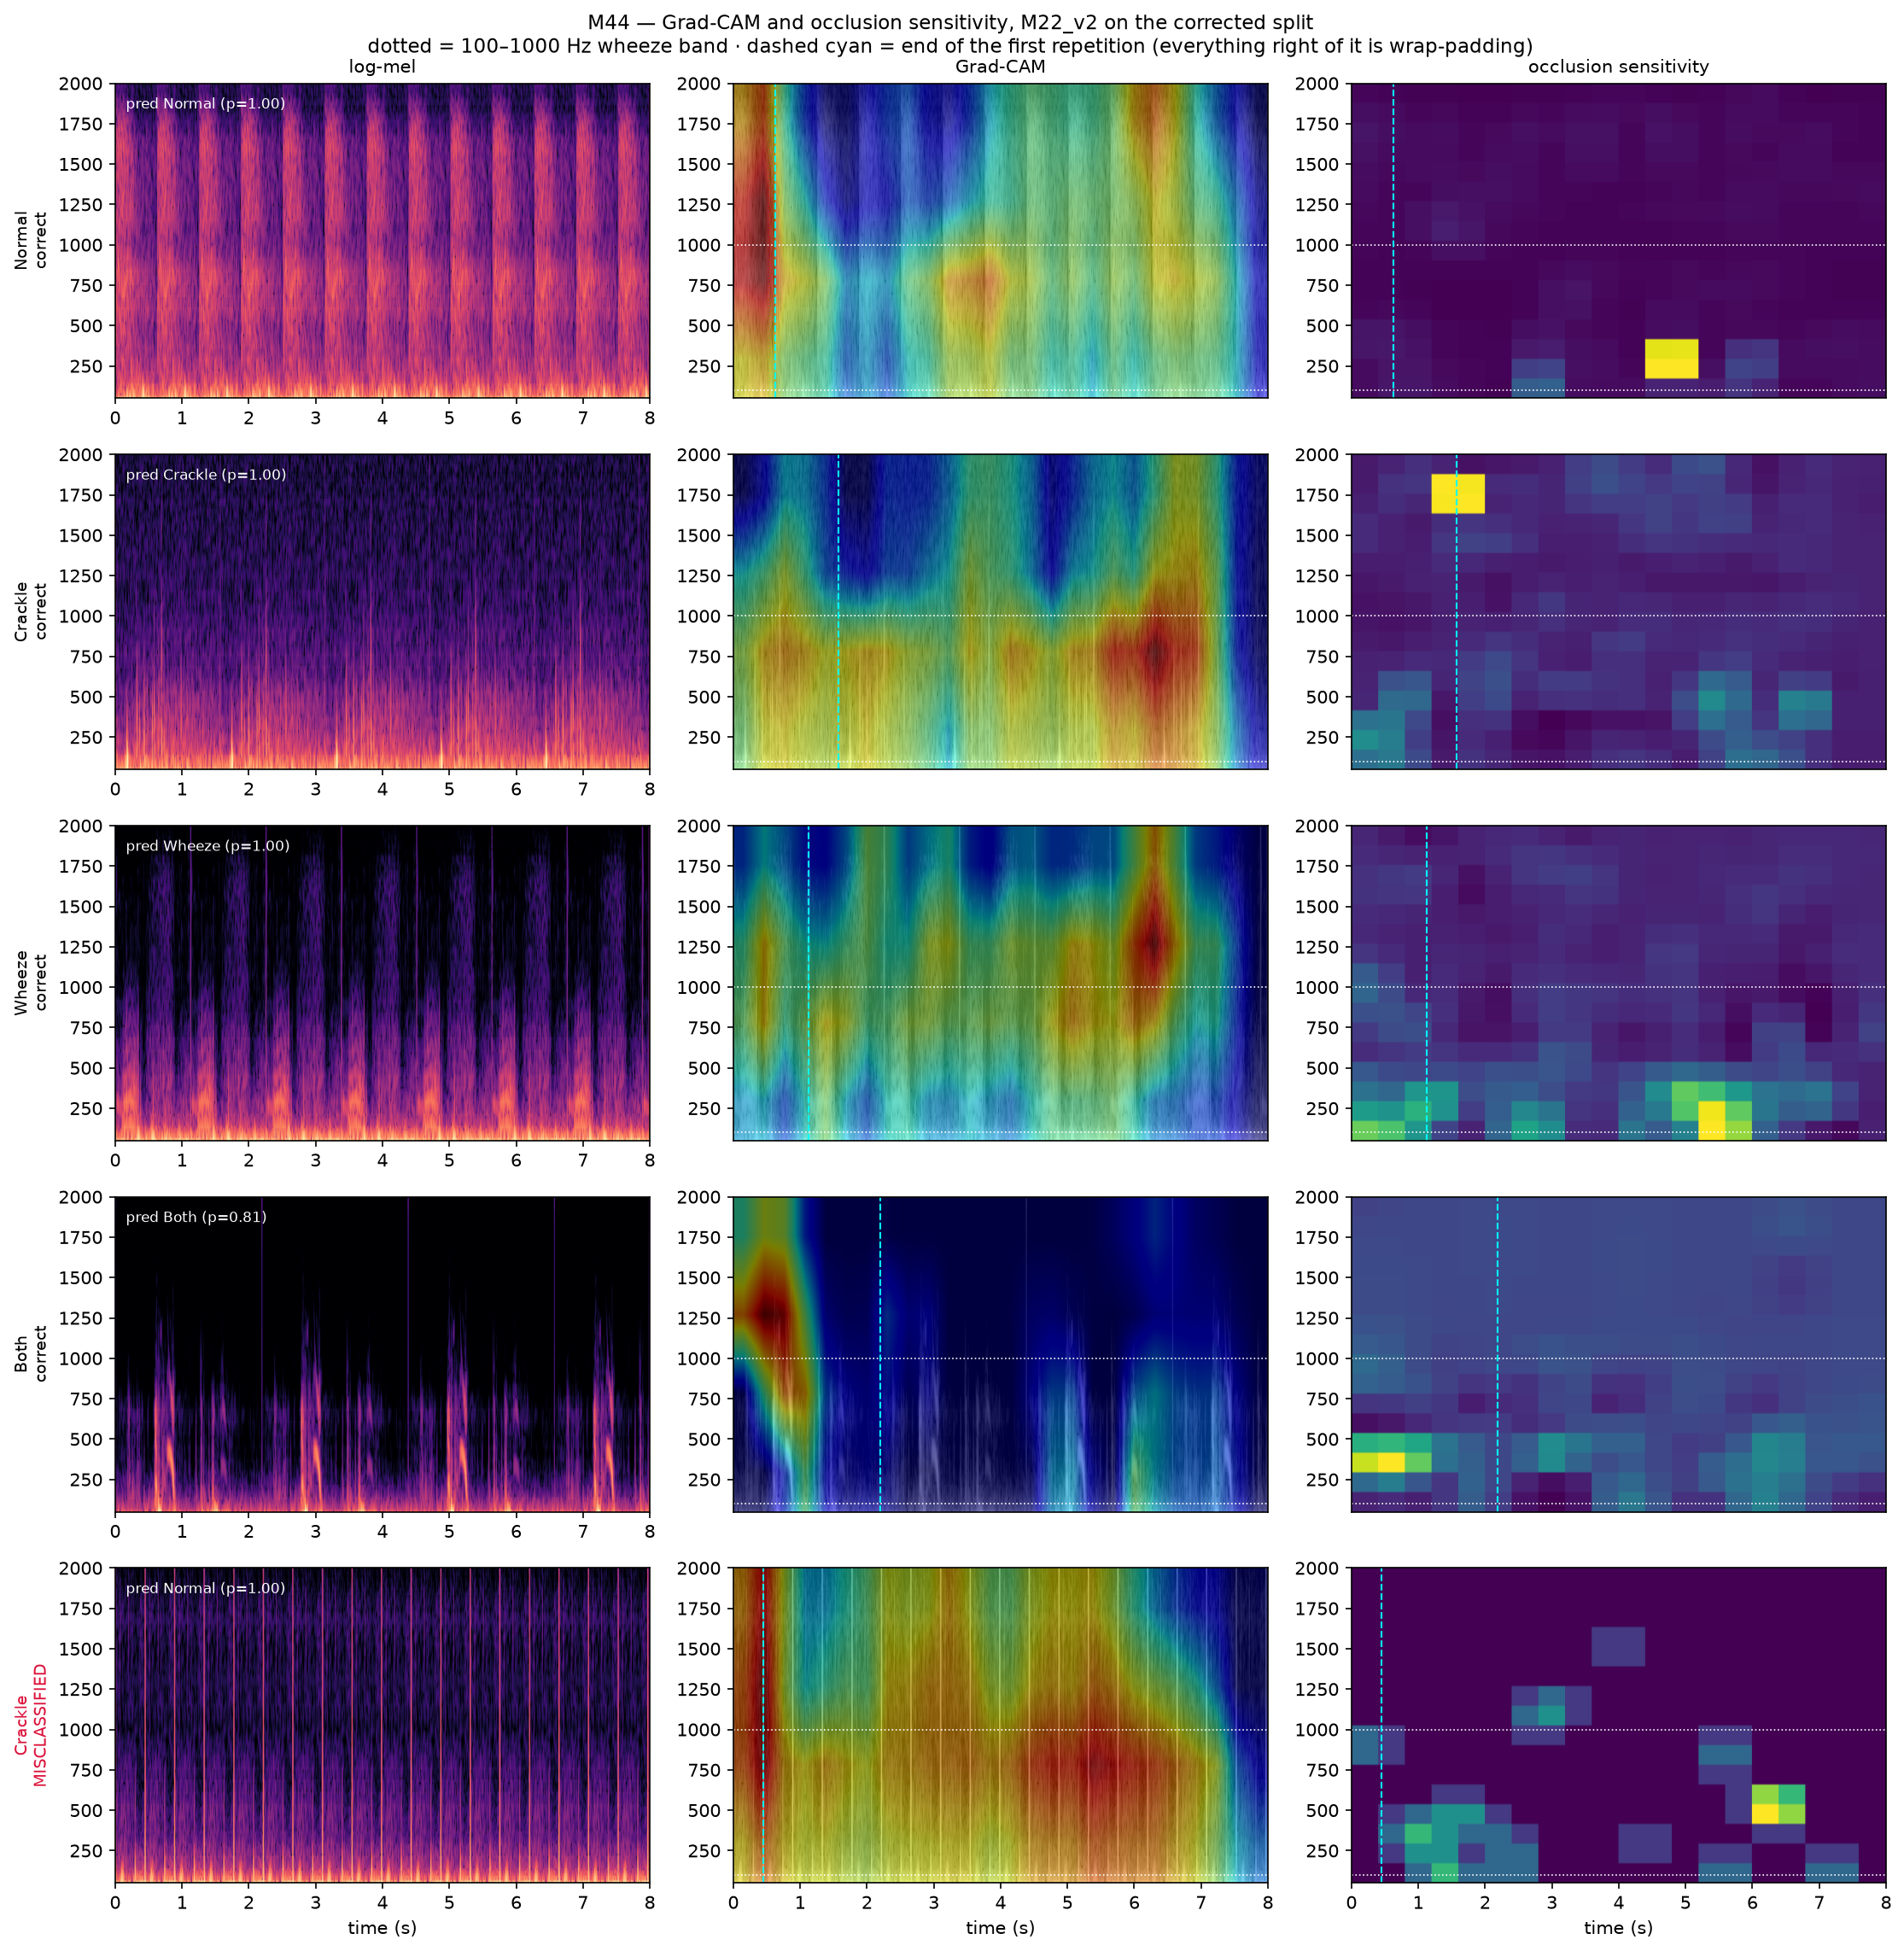
\includegraphics[width=0.42\linewidth]{figures/fig_xai_panels.png}
\caption{Attribution for the best model. Each row is one test cycle: the log-mel spectrogram,
the gradient-based attribution, the occlusion map, and the predicted against the true label.
The bottom row is a misclassified cycle.}
\label{fig:xai}
\end{figure}

\begin{table}[!t]
\centering
\caption{Quantitative explainability, each row a measurement with an interval rather than a
description of a picture. Band pointing asks whether attribution concentrates in the
100--1000~Hz wheeze band, tiling consistency whether the model attributes alike to the
identical repeated copies of the cycle inside one input, and padding attention how much
attribution falls after the real cycle ends.}
\label{tab:xaiquant}
\footnotesize
\begin{tabular}{llrl}
\toprule
Measure & Condition & Value & Reading \\
\midrule
\multirow{4}{*}{Band pointing}
 & uniform baseline & 0.5547 & what an unfocused map would give \\
 & wheeze absent ($n = 325$) & 0.7674 & concentrates in the band \\
 & wheeze present ($n = 75$) & 0.7140 & concentrates \emph{less} \\
 & \best{difference} & \best{$-0.0534$} & [$-$0.0785, $-$0.0256], $p = 0.001$ \\
\midrule
\multirow{3}{*}{Tiling consistency}
 & mean correlation ($n = 361$) & 0.098 & attribution differs across identical audio \\
 & median correlation & 0.180 & --- \\
 & fraction above 0.5 & 32.1\% & only a third are consistent \\
\midrule
\multirow{2}{*}{Padding attention}
 & cyclic tiling, observed / uniform & 0.594 / 0.679 & ratio 0.87 \\
 & zero padding, observed / uniform & 0.101 / 0.679 & ratio 0.15 \\
\bottomrule
\end{tabular}

\vspace{2pt}
\footnotesize A resolution caveat travels with the gradient maps. MobileNetV2 downsamples by
32, so its final convolutional block is 4 frequency by 26 time cells---roughly 500~Hz and
0.31~s each---and every map in Fig.~\ref{fig:xai} is that grid interpolated up to
$128 \times 801$. The \emph{direction} of both measurements is trustworthy because both
intervals exclude their null; the fine structure is interpolation, not measurement. Where the
two maps disagree, prefer occlusion: its grid is 16 mel bins by 80 frames and needs no gradient
through a downsampled layer.
\end{table}

Both quantitative results run against the story the score tells.

The band-pointing result is backwards. The model does concentrate on the physiological band in
general---both groups sit well above the uniform baseline---but when a wheeze is actually
present it attends to that band \emph{less}, with the interval on that difference comfortably
clear of zero. A wheeze detector should show the opposite contrast.

The tiling result is the one that changed the paper. Every cycle shorter than 8~s is repeated
two or three times inside the input, so a model reading acoustics should attribute the same way
to each copy. It does not: mean correlation 0.098, only a third of cycles above 0.5. A
substantial part of the attribution tracks \emph{position in the window} rather than sound.
That is what made us add row \texttt{P4}, which replaces cyclic tiling with zero padding, and
the padding-attention rows show the two models behaving completely differently in the padded
region. \texttt{P4} costs 0.0311, so tiling is doing real work; whether that work is acoustic
or positional these measurements do not settle, and we do not claim otherwise.

We deliberately do not call any of this clinical validation, and this is where our reading of
Bikku \emph{et al.}~\cite{scirep2025cnnrnn} shows up in our own method: the labels these
attributions are aligned to are reproduced by a physician at $\kappa = 0.035$ on crackles, so a
map aligned to them tells you where a model looks, not that it reasons like a clinician. One
planned analysis was dropped rather than faked. We had intended a pointing game asking whether
attribution mass lands inside the annotated event window, but ICBHI annotates \emph{whether} a
cycle contains an adventitious sound and not \emph{where}, and the pipeline crops to exactly
that window, so the hit rate is 100 percent by construction.

\subsection{Statistical Analysis}
\label{subsec:stats}

Two questions have to be answered before any ablation delta can be believed: how large is
run-to-run noise, and what is the effective sample size. Table~\ref{tab:stats} answers both.

\begin{table}[!t]
\centering
\caption{Statistical analysis. The upper block is one configuration trained three times with
nothing but the seed changed; the lower block tests ten ablation rows twice, by McNemar over
2,636 cycles and by paired bootstrap over 47 patients. Effect sizes are in
Table~\ref{tab:ablation}.}
\label{tab:stats}
\footnotesize
\begin{tabular}{llrrl}
\toprule
\multicolumn{5}{l}{\emph{Noise floor: identical configuration, three seeds}}\\
\multicolumn{2}{l}{Seed 42 / 1 / 2} & \multicolumn{3}{l}{0.5540 / 0.5681 / 0.5657} \\
\multicolumn{2}{l}{Mean, standard deviation, range} & \multicolumn{3}{l}{0.5626, \best{0.0075}, \best{0.0141}} \\
\midrule
\multicolumn{5}{l}{\emph{Unit of analysis: the same ten rows tested two ways}}\\
Row & Patient-level 95\% CI on the difference & Patient $p$ & Cycle $p$ & Units agree? \\
\midrule
\texttt{C2} random init      & [$-$0.130, $+$0.003] & 0.0625 & $<0.001$ & no \\
\texttt{C3} plain CE         & [$-$0.049, $+$0.023] & 0.5625 & 0.150 & yes \\
\texttt{C4} frozen backbone  & [$-$0.154, $-$0.052] & \best{$<0.001$} & $<0.001$ & yes \\
\texttt{C5} 64 mel bins      & [$-$0.061, $+$0.020] & 0.3915 & 0.026 & no \\
\texttt{C6} 4~s cycles       & [$-$0.092, $+$0.009] & 0.1265 & $<0.001$ & no \\
\texttt{P1} + band-pass      & [$-$0.059, $+$0.034] & 0.6860 & 0.128 & yes \\
\texttt{P2} + denoising      & [$-$0.089, $+$0.011] & 0.1380 & $<0.001$ & no \\
\texttt{P3} + amplitude norm & [$-$0.017, $+$0.046] & 0.3670 & 0.040 & no \\
\texttt{P4} zero padding     & [$-$0.068, $+$0.006] & 0.0955 & $<0.001$ & no \\
\texttt{P5} $-$ min--max     & [$-$0.041, $+$0.027] & 0.7170 & 0.428 & yes \\
\midrule
\multicolumn{2}{l}{\emph{Significant at the 0.05 level}} & \best{1 of 10} & \best{7 of 10} & 6 rows flip \\
\bottomrule
\end{tabular}
\end{table}

The reference value of 0.5602 sits inside the seed band, which doubles as an unplanned
reproducibility check: the replicates came from a different harness than the notebook that
produced the reference, and the two implementations agree to within run-to-run noise. Read
against that range, three of eleven ablation deltas do not clear it---removing class weighting,
adding a band-pass filter, removing the min--max rescale---two more clear it by less than a
factor of 1.25 and are not safe alone, and the remaining six clear it by at least 2.2.

The lower block says something different and equally important. The corrected test partition
holds 2,636 cycles but only 47 patients, and cycles from one patient are not independent:
testing per cycle makes seven of ten rows significant, testing per patient makes one, and six
rows change verdict depending on the unit. The two blocks do not contradict each other. The
seed band says run-to-run noise is too small to explain most of these deltas; the patient-level
test says this test set is too small to certify them. Most of the effects are probably real,
and this benchmark cannot prove it.

\subsection{Ablation Study}
\label{subsec:ablation}

The ablation runs on the best model, on the corrected partition, changing one thing per row.
Table~\ref{tab:ablation} has twelve rows: seven that remove or replace a model component and
five that switch a preprocessing stage. Rows \texttt{P1} to \texttt{P3} \emph{add} a stage the
reference does not have, so their sign reads the other way---a positive delta there is a
recommendation to adopt.

\begin{table}[!t]
\centering
\caption{Component and preprocessing ablation on the best model, corrected partition, one
variable per row. Intervals are 95 percent patient-level bootstrap. The last column gives each
delta as a multiple of the measured noise range of 0.0141. The reference and \texttt{C1} come
from the training notebooks; every other row comes from the ablation harness, which reuses the
same settings---see the note below.}
\label{tab:ablation}
\footnotesize
\begin{tabular}{llrlrrrl}
\toprule
Row & Change from the reference & ICBHI & 95\% CI & $\Delta$ & $S_e$ & $S_p$ & vs noise \\
\midrule
\texttt{REF} & MobileNetV2 + SpecAugment & \best{0.5602} & [0.508, 0.614] & --- & 0.4089 & 0.7115 & --- \\
\texttt{C1} & $-$ SpecAugment & 0.5200 & [0.463, 0.575] & $-0.0402$ & 0.4266 & 0.6135 & $2.9\times$ \\
\texttt{C2} & $-$ ImageNet pretraining & 0.4999 & [0.438, 0.551] & $-0.0603$ & 0.3736 & 0.6263 & $4.3\times$ \\
\texttt{C3} & $-$ class-weighted loss & 0.5497 & [0.502, 0.593] & $-0.0105$ & 0.4275 & 0.6718 & \emph{below} \\
\texttt{C4} & frozen backbone, head only & 0.4595 & [0.400, 0.521] & $-0.1007$ & 0.4349 & 0.4840 & $7.1\times$ \\
\texttt{C5} & 64 mel bins instead of 128 & 0.5427 & [0.492, 0.587] & $-0.0175$ & 0.4238 & 0.6615 & $1.2\times$ \\
\texttt{C6} & 4~s cycles instead of 8~s & 0.5224 & [0.463, 0.574] & $-0.0378$ & 0.4954 & 0.5494 & $2.7\times$ \\
\texttt{C7} & random init \emph{and} frozen & 0.4979 & --- & $-0.0623$ & 0.0028 & 0.9929 & $4.4\times$ \\
\midrule
\texttt{P1} & $+$ band-pass filter & 0.5513 & [0.492, 0.601] & $-0.0089$ & 0.4442 & 0.6583 & \emph{below} \\
\texttt{P2} & $+$ spectral-gating denoising & 0.5248 & [0.458, 0.588] & $-0.0354$ & 0.4572 & 0.5923 & $2.5\times$ \\
\texttt{P3} & $+$ per-cycle amplitude norm. & \best{0.5764} & [0.514, 0.632] & $+0.0162$ & 0.3996 & 0.7532 & $1.1\times$ \\
\texttt{P4} & zero padding instead of tiling & 0.5291 & [0.478, 0.581] & $-0.0311$ & 0.4684 & 0.5897 & $2.2\times$ \\
\texttt{P5} & $-$ min--max rescale & 0.5539 & [0.501, 0.604] & $-0.0063$ & 0.4136 & 0.6942 & \emph{below} \\
\bottomrule
\end{tabular}

\vspace{2pt}
\footnotesize Two implementations meet in this table and the reader should know it. Run on the
reference configuration at seed 42, the ablation harness returns 0.5540 against the notebook's
0.5602. The difference sits inside the run-to-run range of Table~\ref{tab:stats}, which is what
licenses reading the two as one table, and it is also why we treat any delta below that range
as unresolved rather than as a small effect.
\end{table}

Four results here are worth arguing about.

\emph{Fine-tuning matters far more than pretraining.} Freezing the backbone costs 0.1007, the
largest single effect and the only row that survives the patient-level test; random
initialisation costs 0.0603. Both were expected. \texttt{C7} was not: it does both at once.
Freezing a \emph{random} backbone scores 0.4979 while freezing the \emph{ImageNet} backbone
scores 0.4595, so frozen ImageNet features are 0.038 worse than random projections on log-mel
spectrograms, 2.7 times the noise range. Transfer from images to spectrograms only pays once
the backbone can move, and until then it is actively harmful. That decomposes \texttt{C4} into
two statements---pretraining is worthless frozen, and adaptation is what the 0.10 buys---and
neither \texttt{C2} nor \texttt{C4} could produce it alone.

\emph{The three preprocessing stages we never had were mostly not missing.} Band-pass filtering
is neutral, denoising costs 0.0354, and only amplitude normalisation helps, at $+0.0162$.
Denoising is the interesting one: spectral gating removes stationary noise, and crackles are
short transients whose detectability depends on exactly the low-energy structure it
suppresses.

\emph{The highest score in the table is not the model we report.} \texttt{P3} reaches 0.5764,
above the reference, and we do not promote it: its delta is 1.1 times the noise range and its
patient-level interval spans zero. Promoting it would be the same class of mistake this paper
is about, made with our own evidence in front of us. \emph{Class weighting, meanwhile, barely
matters}---removing it costs 0.0105, below the noise floor, so the standard answer to the
imbalance is worth less here than the padding scheme.

The table above is leave-one-out. We also assembled the cumulative form, which exposes an
ordering effect a single ordering would hide: added after masking, class weighting is credited
$+0.0105$, while added after class weighting, masking is credited $+0.0402$, and the two agree
only at the end point. Its bottom three rungs need GPU runs we did not complete and are recorded
as \notrun\ rather than filled with plausible values.

Table~\ref{tab:ablationreason} restates the single largest controllable component one metric at
a time, because a composite delta hides opposite movements in sensitivity and specificity.

\begin{table}[!t]
\centering
\caption{Metric-by-metric ablation of spectrogram masking on the best model. Configuration A is
the clean control and configuration B adds masking; nothing else differs, including the seed.}
\label{tab:ablationreason}
\footnotesize
\begin{tabular}{lrrrl}
\toprule
Metric & A: no masking & B: + masking & Progress & Possible reason \\
\midrule
Accuracy    & 0.5372 & 0.5880 & $+9.46\%$  & fewer Normal cycles called abnormal \\
Precision   & 0.3917 & 0.4322 & $+10.34\%$ & masking suppresses over-firing on rare classes \\
Recall      & 0.4091 & 0.4103 & $+0.29\%$  & essentially unchanged; masking adds no coverage \\
F1-score    & 0.3985 & 0.4141 & $+3.91\%$  & precision gain with recall flat \\
Sensitivity & 0.4266 & 0.4089 & $-4.15\%$  & the model becomes more conservative on abnormal cycles \\
Specificity & 0.6135 & 0.7115 & $+15.97\%$ & the whole gain sits here \\
\best{ICBHI score} & 0.5200 & \best{0.5602} & \best{$+7.73\%$} & specificity gain outweighs the sensitivity loss \\
\bottomrule
\end{tabular}
\end{table}

The reason column is the point of that table. Masking does not make the model hear more;
sensitivity actually falls. It makes the model stop calling Normal cycles abnormal, and because
the challenge metric weights sensitivity and specificity equally, a 16 percent specificity gain
against a 4 percent sensitivity loss reads as progress. On a screening application where missed
abnormalities are the expensive error, the same change might be a regression.

\subsection{Failure Analysis}
\label{subsec:failures}

Eight runs failed outright, and every one was caught by an automated check over the committed
result files rather than by inspection. A sensitivity or specificity floor caught four
collapses: the ViT run at $S_e = 0.0000$, the first temporal transformer at $S_p = 0.0000$, the
distillation run at $S_e = 0.0932$ and the acoustic curriculum run at $S_e = 0.0186$. A
selection-sanity check caught the repeated physics-informed run, whose best epoch was its
first. A chance-level check caught the OpenMax baseline at AUROC 0.4516, which invalidates every
comparison against it. A verifiability check caught a run reporting a challenge score with no
confusion matrix---the defect that also keeps the Audio Spectrogram Transformer out of
Table~\ref{tab:metricaudit}.

The eighth is our favourite. One run reported that temperature scaling raised its accuracy from
0.3573 to 0.6595. Temperature scaling is a monotone transform of the logits, so it cannot change
which class scores highest and therefore cannot change accuracy at all. That run was reporting
something which cannot happen, and a three-line assertion catches it.

\subsection{Limitations}
\label{subsec:limitations}

Six things constrain what this paper can claim, and we would rather state them than have them
found. The most serious is that our training loop monitors the test partition each epoch: there
is no separate validation split in the ablation harness, so ``select the best epoch'' means
select on test. Every score in Table~\ref{tab:ablation} carries that advantage equally, and the
deltas between rows are what survive it; Table~\ref{tab:selection} prices the rule at 0.075 to
0.102, a lower bound on what a clean protocol would cost us. Second, the one audio-pretrained
transformer predates the audit, sits on the wrong partition under the wrong metric with
different preprocessing, and committed no confusion matrix, so the most informative comparison
in the paper---image against audio pretraining under one protocol---is the one we cannot
make. Third, the ViT collapse is reported as a small-data finding, but we never tried a warm-up
schedule with a lower backbone learning rate, which is the standard remedy, so it may be a
schedule artefact and ours is the weaker claim. Fourth, the split effect is measured on one
model chain only; two earlier runs appear to show larger split effects, but those pairs differ
in architecture as well as partition, so we never quote them. Fifth, there is one clinician, so
no inter-rater agreement is computable---the intra-rater duplicates and the replication of a
published seven-physician sensitivity mitigate this but do not remove it. Sixth, everything here
is one corpus, so the scope of every claim is ICBHI 2017.

\subsection{Comparison with Existing Works}
\label{subsec:comparison}

Table~\ref{tab:comparison} places our system against published work. We report the challenge
metric only, and the partition for every row, because the argument of this paper is that a
comparison missing those two columns is not a comparison.

\begin{table}[!t]
\centering
\caption{Comparison against published systems on ICBHI 2017, all under the challenge metric
of~(\ref{eq:official}). Rows in different blocks sit on different partitions and are not
rankable against one another.}
\label{tab:comparison}
\footnotesize
\begin{tabular}{lllrrr}
\toprule
Author & Dataset & Network & $S_e$ & $S_p$ & \best{ICBHI} \\
\midrule
\multicolumn{6}{l}{\emph{Published 60/40 partition, directly comparable}}\\
Gairola \emph{et al.}~\cite{respirenet2021} & ICBHI 2017 & ResNet34, ImageNet & 0.401 & 0.723 & 0.5620 \\
Moummad and Farrugia~\cite{scl2023} & ICBHI 2017 & CNN6, supervised contrastive & 0.392 & 0.760 & 0.5755 \\
Niizumi \emph{et al.}~\cite{frozenfm2025} & ICBHI 2017 & M2D, frozen linear probe & 0.466 & 0.722 & 0.5938 \\
Bae \emph{et al.}~\cite{bae2023patchmix} & ICBHI 2017 & AST, patch-mix contrastive & 0.431 & 0.817 & 0.6237 \\
Kim \emph{et al.}~\cite{bts2024} & ICBHI 2017 & CLAP, text-aided & 0.457 & 0.814 & 0.6354 \\
Jeong \emph{et al.}~\cite{pafa2025} & ICBHI 2017 & BEATs, patient-aware alignment & 0.476 & 0.821 & \best{0.6484} \\
Tzeng \emph{et al.}~\cite{tzeng2025jmir} & ICBHI 2017 & 7 senior physicians & 0.232 & 0.723 & 0.4777 \\
\addlinespace
\best{This work} & ICBHI 2017 & MobileNetV2 + SpecAugment & 0.456 & 0.672 & \best{0.5641} \\
\best{This work} & ICBHI 2017 & MobileNetV3-Small & 0.198 & 0.828 & 0.5132 \\
\best{This work} & ICBHI 2017 & 2D-CNN from scratch & 0.201 & 0.744 & 0.4720 \\
\midrule
\multicolumn{6}{l}{\emph{Corrected patient-independent partition, not comparable to the block above}}\\
\best{This work} & ICBHI 2017 & MobileNetV2 + SpecAugment & 0.409 & 0.712 & \best{0.5602} \\
\best{This work} & ICBHI 2017 & Swin-T & 0.343 & 0.718 & 0.5304 \\
\best{This work} & ICBHI 2017 & DeiT-S & 0.295 & 0.735 & 0.5149 \\
\best{This work} & ICBHI 2017 & ViT-B/16, collapsed & 0.000 & 0.999 & 0.4994 \\
\midrule
\multicolumn{6}{l}{\emph{Identifier-fallback partition, shown only to price the fault}}\\
This work & ICBHI 2017 & MobileNetV2 + SpecAugment & 0.570 & 0.729 & 0.6495 \\
This work & ICBHI 2017 & the same run, macro metric & 0.570 & 0.729 & 0.7077 \\
This work & ICBHI 2017 & AST, macro metric, \notrec\ officially & --- & --- & 0.6359 \\
\bottomrule
\end{tabular}

\vspace{2pt}
\footnotesize Published rows use the official partition, 2,756 test cycles from 49 patients; our
first block is that identical partition and metric, which is why it is the only block of ours
that may be read against them. The last row is the pre-audit Audio Spectrogram Transformer,
placed here because its only surviving score is the macro variant. Three works cited elsewhere
are absent because none reports a number this table can hold: Suma
\emph{et al.}~\cite{suma2025mtl} give accuracy on an unstated partition, Bikku
\emph{et al.}~\cite{scirep2025cnnrnn} accuracy under five-fold cross-validation, and Cho and
Lee~\cite{cho2025openset} an improvement over a baseline. Excluding them applies this paper's
own rule to its own table.
\end{table}

On the partition the literature actually uses, our best model reaches 0.5641, just above
RespireNet---the strongest ImageNet-pretrained convolutional system in the table---and below
every audio-pretrained one, about 8 points short of the best row.

The composite hides the more useful comparison, and this is the concrete payoff of the
reporting discipline of Section~\ref{subsec:protocol}. \emph{Our sensitivity is not behind the
field.} At 0.456 it beats RespireNet (0.401), supervised contrastive pretraining (0.392) and
patch-mix contrastive learning (0.431), sits level with the text-aided CLAP system (0.457), and
trails only the frozen probe (0.466) and the best BEATs system (0.476). The whole deficit is
specificity: 0.672 against a field between 0.722 and 0.821. We are not uniformly weaker, we sit
at a different operating point---finding abnormal cycles at roughly the field's rate while
over-calling them on normal ones, which is the direction a class-weighted loss and spectrogram
masking push a model by design, and arguably the direction a screening tool should prefer.
Under the composite alone the distinction vanishes.

The last three rows are the ones this paper exists for. Our unaudited pipeline reported 0.7077,
which would have placed first in this table, ahead of every published system, on a partition
covering 7.1 percent of the corpus under a metric we had defined ourselves. It was not state of
the art, it was an unaudited measurement. A 2.2~M-parameter MobileNetV2 landing level with a
2021 ResNet34 is an ordinary outcome for a course project; finding out why the same code first
said otherwise is not.

%=======================================================================
\section{Conclusions}
\label{sec:conclusion}

We set out to build an interpretable open-world respiratory sound classifier and ended up
building an audit. The turn came from a gate written down in advance: our concept detectors had
to reproduce ICBHI's crackle and wheeze labels above 0.65, they reached 0.5580 and 0.5340 over
two runs, and the rule said stop. Looking for an explanation sent us into our own evaluation
code, where we found five faults. A macro-averaged score variant inflated 20 runs by 0.0948 on
average; a split loader silently fell back to an 11-patient test set worth 0.0893; the published
split assigns recordings rather than patients, though repairing that leak is worth only 0.0039;
one recording's device suffix does not match the released audio; and selecting the checkpoint by
minimum loss rather than by the challenge score costs 0.0752 to 0.1015 across three seeds. Our
unaudited pipeline reported 0.7077 where the corrected one reports 0.5602, and that 0.1475 is
larger than every architectural choice in this paper put together.

Under the corrected protocol MobileNetV2 with spectrogram masking is our best model, at 0.5602
on the corrected partition and 0.5641 on the published one, with 2.2~M parameters. All three
vision transformers lost to it and ViT-B/16 collapsed to the majority class at 38 times the
parameter count, while the one audio-pretrained transformer cannot be placed beside them at all
because it predates the audit and stored no prediction table---the paper's own argument,
demonstrated on its own most interesting model. The ablation says fine-tuning is worth far more
than pretraining, that frozen ImageNet features are measurably \emph{worse} than random
projections on log-mel input, that masking buys specificity rather than sensitivity, and that
class weighting is worth less than the padding scheme---though a three-seed noise floor of
0.0141 rules three of those deltas inadmissible and a patient-level test over 47 patients
certifies only one. The concept branch ended in a retraction: a pre-registered probe on a frozen
AudioSet embedding reaches 0.7115 and 0.7621 on the very cycles our detectors failed on, so the
labels support strong detection and our extractors were weak. What replaced the claim is
better---on the same 132 clips that machine reproduces ICBHI's wheeze labels more closely than a
self-consistent physician does, by 0.169 at $p = 0.046$.

The practical recommendation is short. Report the challenge metric with sensitivity and
specificity beside it, name the partition and say whether it is patient-independent, commit the
raw confusion matrix, state the checkpoint selection rule, and test over patients rather than
cycles. Four of the five faults are invisible without those habits, all five sat in code that
ran without error, and the third is the one whose absence cost us an entire model.

Three things follow from what is unfinished. \emph{A clean validation protocol, and the fourth
transformer re-run:} our harness monitors the test partition every epoch, so every score here
carries a selection advantage; carving a validation split from the 79 training patients would
remove it, at a cost Table~\ref{tab:selection} puts at 0.075 to 0.102, and the audio-pretrained
transformer belongs in the same batch as the one experiment that tests the pretraining-domain
hypothesis directly. \emph{A reference standard built for the task:} a multi-rater re-annotation of even a few
hundred cycles, with calibration exemplars and an explicit ``fits no named category'' option,
would separate model error from label noise---our own pack found roughly 7 percent of clips
containing a sound fitting none of the four named classes.
\emph{Fine-tuning that preserves what pretraining learned:} the frozen probe in
Table~\ref{tab:ceiling} recovers these labels at 0.71 and 0.76 with no task training, while our
ImageNet backbones are useless until allowed to move. Whether adaptation can be constrained so
that it keeps the acoustic structure a large audio model already carries is a concrete next
step, and the probe supplies its success criterion.

Two habits made this project worth writing up: fix the threshold before running the experiment,
and audit your own pipeline before you audit anyone else's.

%=======================================================================
\appendices
\section{Run Identifier Map}
\label{app:runmap}

Models are named by architecture throughout the paper. During development they carried short
internal identifiers, and those identifiers are what the repository's result files are named
after. Table~\ref{tab:runmap} maps one to the other so that every number above can be traced to
the file it came from.

\begin{table}[!h]
\centering
\caption{Internal run identifiers, the name used in this paper, and where each is reported.}
\label{tab:runmap}
\footnotesize
\begin{tabular}{lll}
\toprule
Identifier & Name in this paper & Reported in \\
\midrule
M22-v2 & MobileNetV2 + SpecAugment --- the reference and best model & Tables~\ref{tab:main}--\ref{tab:comparison} \\
M3-v2 & MobileNetV2, clean control, ablation row \texttt{C1} & Tables~\ref{tab:main}, \ref{tab:ablation} \\
M40, M41, M42 & ViT-B/16, Swin-T, DeiT-S & Tables~\ref{tab:main}, \ref{tab:efficiency}, \ref{tab:comparison} \\
M4 / M43 & AST pre-audit / its corrected re-run (\notrun) & Section~\ref{subsec:ast} \\
M1, M2, M3, M12, M22 & the pre-audit backbone line and its selection study & Tables~\ref{tab:metricaudit}, \ref{tab:protocol}, \ref{tab:comparison} \\
M7 & MobileNetV2 ensemble, $N = 5$ & Section~\ref{subsec:augmentation} \\
M6, M29 & OpenMax and post-hoc energy open-set baselines & Sections~\ref{subsec:extensions}, \ref{subsec:failures} \\
M30--M37 & the extension sweep & Tables~\ref{tab:metricaudit}, \ref{tab:extensions} \\
M39 & physics-derived concept extraction and the gate & Table~\ref{tab:gate} \\
M44, M45 & interpretability analysis; component and preprocessing ablation & Tables~\ref{tab:xaiquant}, \ref{tab:ablation} \\
M48 & protocol ablation, seed band, same-clips comparison & Tables~\ref{tab:selection}, \ref{tab:protocol}, \ref{tab:human}, \ref{tab:stats} \\
N11 & supervised ceiling estimate & Table~\ref{tab:ceiling} \\
\bottomrule
\end{tabular}
\end{table}

%=======================================================================
\bibliographystyle{IEEEtran}
\bibliography{references}

\end{document}
